\documentclass[mscthesis, 12pt, a4paper, oneside]{usiinfthesis}
\usepackage{float}
\usepackage{lipsum}
\usepackage{graphicx}
\usepackage[acronym, toc]{glossaries}
\usepackage{listings}
\usepackage{breqn}
\usepackage{subfig}
\usepackage{csquotes}
\usepackage[shortlabels, inline]{enumitem}
\usepackage[normalem]{ulem}
\useunder{\uline}{\ul}{}

\DeclareMathOperator*{\argmax}{arg\,max}
\DeclareMathOperator*{\argmin}{arg\,min}


\makeatletter
\patchcmd\eq@setnumber{\stepcounter}{\refstepcounter}{}{%
  \errmessage{Patching \noexpand\eq@setnumber failed}%
}
\makeatother


\lstdefinelanguage{algebra}
{morekeywords={import,sort,constructors,observers,transformers,axioms,if,
else,end},
sensitive=false,
morecomment=[l]{//s},
}


\title{Active Learning for Visual Anomaly Detection Applied to Mobile Robots} %compulsory
\specialization{Artificial Intelligence}%optional
%\subtitle{Subtitle: A modern \textbf{Active Learning} approach} %optional 
\author{Alind Xhyra} %compulsory
\begin{committee}
\advisor{Prof.}{Alessandro Giusti}{Advisor} %compulsory
\coadvisor{}{Dario Mantegazza}{Co-Advisor}{} %optional
\coadvisor{Prof.}{Domenico Giorgio Sorrenti}{Co-Advisor}{} %optional
\end{committee}
\Day{27} %compulsory
\Month{October} %compulsory
\Year{2022} %compulsory, put only the year
\place{Lugano} %compulsory

% \dedication{To my beloved} %optional
\openepigraph{\enquote{A computer would deserve to be called intelligent if it could deceive a human into believing that it was human.}}{Alan Turing} %optional

%\makeindex %optional, also comment out \theindex at the end
\newglossaryentry{latex}
{
        name=latex,
        description={Is a mark up language specially suited for 
scientific documents}
}

\newglossaryentry{maths}
{
        name=mathematics,
        description={Mathematics is what mathematicians do}
}

\newglossaryentry{formula}
{
        name=formula,
        description={A mathematical expression}
}

\newacronym{cnn}{CNN}{Convolutional Neural Network}

\newacronym{gcd}{GCD}{Greatest Common Divisor}

\newacronym{lcm}{LCM}{Least Common Multiple}

\newacronym{al}{AL}{Active Learning}

\newacronym{ml}{ML}{Machine Learning}

\newacronym{idsia}{IDSIA}{Istituto Dalle Molle di Studi sull'Intelligenza Artificiale}

\newacronym{usi}{USI}{Università della Svizzera Italiana}

\newacronym{mse}{MSE}{Mean Squared Error}

\newacronym{mae}{MAE}{Mean Absolute Error}

\newacronym{lc}{LC}{Least Confidence}

\newacronym{ms}{MS}{Margin Sampling}

\newacronym{en}{EN}{Entropy}

\newacronym{bald}{BALD}{Bayesian Active Learning by Disagreement}

\newacronym{mc}{MC}{Monte Carlo}

\newacronym{ceal}{CEAL}{Cost-Effective Active Learning}

\newacronym{gan}{GAN}{Generative Adversarial Network}

\newacronym{ae}{AE}{Autoencoder}

\newacronym{cae}{CAE}{Convolutional Autoencoder}

\newacronym{dl}{DL}{Deep Learning}

\newacronym{ad}{AD}{Anomaly Detection}

\newacronym{ssh}{SSH}{Secure SHell}

\newacronym{ap}{AP}{Access Point}

\newacronym{fps}{FPS}{Frames Per Second}

\newacronym{fov}{FOV}{Field Of View}

\newacronym{ros}{ROS}{Robot Operating System}

\newacronym{api}{API}{Application Programming Interface}

\newacronym{pdf}{pdf}{Probability Density Function}

\newacronym{iid}{i.i.d.}{Indipedent and Identically Distributed}

\newacronym{oe}{OE}{Outlier Exposure}

\newacronym{auc}{AUC}{Area Under the Curve}

\newacronym{tpr}{TPR}{True Positive Rate}

\newacronym{fpr}{FPR}{False Positive Rate}

\newacronym{tnr}{TNR}{True Negative Rate}

\newacronym{fnr}{FNR}{False Negative Rate}

\newacronym{tp}{TP}{True Positive}

\newacronym{fp}{FP}{False Positive}

\newacronym{tn}{TN}{True Negative}

\newacronym{fn}{FN}{False Negative}

\newacronym{roc}{ROC}{Receiver Operating Characteristic}

\newacronym{nn}{NN}{Nearest Neighbor}

\newacronym{vae}{VAE}{Variational Autoencoder}
\makenoidxglossaries


\begin{document}


\maketitle %generates the titlepage, this is FIXED

\frontmatter %generates the frontmatter, this is FIXED

\begin{abstract}



State-of-the-art approaches for visual Anomaly Detection rely on Deep Learning techniques; these techniques require an enormous amount of labeled data for training. This data in some specific fields such as medical imagery, robotics, and safety-critical situations may require expert annotators. Because their time is limited, such labeling is expensive.
\acrfull{al} tries to overcome this issue by choosing from the available unlabeled data only the samples that improve most the knowledge of the model.


We adapt and compare different Active Learning techniques applied to Anomaly Detection tasks for ground mobile robots, using only the robot's camera stream as input. We test them on a proxy task based on the MNIST dataset. We acquire an additional dataset for experimentation by recording a robot's camera feed while it is moving around different corridors on a university campus. The dataset is collected from divers scenarios and stages more more than a dozen types of anomalies. The dataset is composed of more than 40GB of images counting up to 228,795 total frames. We replicate the experiments defined on the collected dataset to check the performance of the \acrshort{al} methods studied.

% \acrfull{dl} approaches to \acrfull{ad} have reached state-of-the-art performance. Such techniques require an enormous amount of labeled data to be available, which in some specific or niche fields such as medical imagery, robotics, and safety-critical situations may require expert annotators. Since their time is limited, relying only on experts for \acrshort{dl} approaches may not be reliable. \acrfull{al} tries to overcome this issue by choosing from the available unlabeled data only the samples that improve the knowledge of the model.

% We propose an autoencoder model for \acrshort{ad} applied to ground mobile robots, using only the robot's camera stream as input. We acquire training and testing datasets for this problem by recording the robot's camera feed while moving around different corridors on the university campus. This system lets us collect data from diverse scenarios and stage more than a dozen types of anomalies, composed by more than 40GB of raw data collected across six environments. We then train an autoencoder on a proxy task based on the MNIST dataset to find and test different model configurations and \acrshort{al} approaches adapted from literature. Once we find the best model setup and metrics, we move to the collected one to check the performance of the \acrshort{al} methods found.



\end{abstract}

% \begin{abstract}[Sommario]

% \end{abstract}

% \begin{acknowledgements}
% \lipsum 
% \end{acknowledgements}

\tableofcontents 
\listoffigures %optional
\listoftables %optional
\lstlistoflistings

\chapter{Introduction}

     \acrfull{ad} problems try to find samples that show an unexpected behavior or pattern given a context of \emph{normality}. These unexpected samples are referred to as \emph{anomalies} or \emph{outliers}.
    \acrshort{ad} applied to mobile robots could be used to solve hazard detection problems without having prior knowledge nor definition of the hazards.
    \\
    
    Recently, a solution \cite{wellhausen2020safe, mantegazza2022outlier} to \acrshort{ad} has been developed using autoencoders. Autoencoders have achieved state-of-the-art performance in the context of visual Anomaly Detection. However, such models require very large amounts of labeled data to be trained and tested on. This labeling can be very expensive in some fields where experts are required (i.e. Medical Images, Robotics, \dots). The goal of \acrfull{al} is to reduce this cost by carefully choosing the \emph{best} samples to be labeled to increase the model performance on the given task.
    \\
    
    This thesis reports the work and research done to implement an \acrshort{al} system applied to the task of \emph{visual anomaly detection} for mobile robots using Undercomplete Convolutional Autoencoders.
    First, we define a \emph{proxy} task based on the MNIST dataset, in which we consider a class as normal and all the others as anomalous. On this task, we compare different \acrshort{al} techniques adapted from literature. Later we compare the results of our model to a realistic dataset gathered using a ground robot.

\newpage
\section*{Thesis structure}
This thesis is structured in the following chapters:

\begin{itemize}
    \item \textbf{\autoref{chap:rel-work}} discusses the background related work about Anomaly Detection, Active Learning, \emph{uncertainty} and \emph{representativeness} metrics;
    \item \textbf{\autoref{chap:prob}} defines our problem and the proposed solution;
    \item \textbf{\autoref{chap:dataset}} explains the hardware and software setup, the models and the dataset used;
    \item \textbf{\autoref{chap:data-coll}} discusses the data collection and labeling process used to expand a real-life dataset;
    \item \textbf{\autoref{chap:experiments}} explains the conducted experiments and the obtained results.
\end{itemize}

% TODO: implementare alla fine

\mainmatter

\chapter{Related work}
\label{chap:rel-work}

In this chapter, we describe the background research conducted. We introduce both \acrfull{ad} and \acrfull{al} and show how they are treated in the literature. We then describe some \acrshort{al} techniques applied to different contexts.
% This chapter describes the background research conducted in literature to find state-of-the-art techniques and metrics applied to \emph{Active Learning}.

\section{Anomaly Detection}
\acrfull{ad}~\cite{ruff2021unifying} is a research field that focuses on finding anomalous observations in mostly nominal data. Its application spans multiple disciplines such as engineering, machine learning, data mining, and statistics. \acrshort{ad} has applications across different domains. Some of the domains are: cyber-security~\cite{ruff2021unifying, liao2013intrusion, xin2018machine}, robotics~\cite{mantegazza2022outlier, wellhausen2020safe}, biomedical imagery~\cite{schlegl2019f}, automatic surveillance systems~\cite{chakravarty2007anomaly}, insurance~\cite{van2016outlier} and finance~\cite{ahmed2016survey} fraud detection, and more~\cite{ruff2021unifying}.
\\
\\
Because \acrshort{ad} is applied to such a broad range of contexts, a general definition of anomaly has to be as vague as possible.
Ruff et al~\cite{ruff2021unifying} define an anomaly as: \enquote{an observation that deviates considerably
from some concept of normality}, while Chandola et al~\cite{chandola2009anomaly} define it as: \enquote{patterns in data that do not conform to expected behavior.}
Both definitions make clear that a concept of \emph{normality} has to be known and modeled to successfully perform \acrshort{ad}.
\\
\\
In this work, we apply \acrshort{ad} to corridor patrolling robots, described in~\autoref{chap:prob}. We use \acrshort{ad} techniques to images coming from the robot's camera. Currently, the state-of-the-art models for image \acrshort{ad} are \acrfull{dl} based models. Generally, these kinds of model training make use of supervised learning approaches. However, anomalous events are \emph{unexpected} and rare phenomena. For this reason, supervised learning approaches are not suitable because of the strong imbalance between the classes. Therefore in this setup unsupervised learning approaches are used. Models training uses normal data only. Their goal is to make the model learn a representation of \emph{normality}.


% In this work, we apply \acrshort{ad} to corridor patrolling robots. We thus work on images. Currently, image \acrshort{ad} is done using \acrshort{dl}-based models which are state-of-the-art for \acrshort{ad} in any field. Generally, \acrshort{dl} models are trained using supervised learning approaches. However, anomalous events are \emph{unexpected} phenomena which happen very rarely, making supervised approaches not suitable because of the strong imbalance between classes. Therefore, \acrshort{ad} models are trained with unsupervised approaches. Models are trained only using normal data and learn a representation of \emph{normality}.

Supervised methods are not suitable for \acrshort{ad} because of this strong class unbalance and difficulty in modeling and formalizing anomalies.
Since anomalous events happen rarely, \emph{unsupervised} models for \acrshort{ad} are used. These models are usually trained on normal data only.
\\

    % \acrshort{ad} methods are usually \emph{unsupervised} because the \emph{anomalies} are most of the times \emph{unexpected} phenomena which happen very rarely, making supervised methods not suitable for these tasks. Since anomalous events happen rarely, models for \acrshort{ad} are trained on normal data.
    % We perform \acrshort{ad} using an autoencoder, described in the next sections.
\subsection{Anomaly Detection in Images}    
   Recently, Sabokrou et al~\cite{Sabokrou_2018_CVPR} propose a novel model for image \acrshort{ad}.
   They build a model composed of an \acrfull{ae} and a \acrfull{cnn}, used as the network discriminator. This model is trained in an adversarial, unsupervised manner.
   The goal of the autoencoder is to learn how to reconstruct the input image after compressing it in such a way as to fool the discriminator. On the other hand, the discriminator has to tell whether or not the image it received is an original sample from the dataset.
   This model is trained on normal samples only. After training, when the model receives an anomalous image, the autoencoder will not be able to reconstruct it correctly. It will distort the anomalies making it simpler for the discriminator to reject the image. 
   
   
   Sarafijanovic et al~\cite{Sarafijanovic2019distance} propose an inception~\cite{Szegedy_2015_CVPR} like \acrfull{cae} and compared it against a \acrshort{cae} in the same \acrshort{ad} task. The inception like \acrshort{ae} combines convolutional filters with different kernel sizes at the same layer. The authors train the model on normal data only. Then instead of calculating the error map, they compute the distance between the pooled output of the bottleneck and its \acrfull{nn} in the same space. The models are tested over classical benchmark computer vision datasets: MNIST~\cite{lecun1998mnist}, Fashion MNIST~\cite{xiao2017fashion}, CIFAR10~\cite{cifar10}, and CIFAR100~\cite{cifar100}. Their inception-like \acrshort{cae} outperformed state-of-the-art models in all tasks, except for Fashion MNIST.
    
\subsection{Visual Anomaly Detection in Robotics}

    \acrshort{ad} is a relevant problem in the context of robotics. It allows robots to find and avoid anomalies such as potential hazards never seen at design time. These hazards could potentially be dangerous or affect the robot's operation, thus detecting an anomaly could be a \emph{critical task} in some situations.
    \\
    \\
    Early works, used an image processing pipeline with image and pattern matching algorithms for the task~\cite{chakravarty2007anomaly}.
    
    More recent works make use of \acrfull{dl} approaches. Christiansen et al~\cite{christiansen2016deepanomaly} propose DeepAnomaly, a modified AlexNet~\cite{alexnet} implementation as solution to an \acrshort{ad} problem for autonomous agricultural vehicles. Their goal is to avoid obstacles. \acrshort{ad} is performed by applying \emph{background subtraction} to some internal layer of the \acrshort{cnn}, obtaining an \emph{anomaly map}.
    
    Wellhausen et al~\cite{wellhausen2020safe} compare three methods for \acrshort{ad} applied to the context of traversability for legged robots. Their goal is to find a safe traversable path for the robot in an unknown environment. They compare an implementation of an \acrshort{ae} with two different models which make use of the encoder part of the \acrshort{ae}: \emph{Deep SVDD} \cite{scime2018multi}, and Real-NVP \cite{ruff2018deep}. In the results, Real-NVP outperformed both the autoencoder and the Deep SVDD model, which scored the worst.

\subsection{Autoencoder}
% \subsubsection{Autoencoder}

Autoencoders~\cite{kramer1991nonlinear} are artificial neural networks used in \emph{unsupervised learning} and \emph{representation learning} settings. In this kind of network, the output layer has the same size as the input one. The autoencoder is trained with the objective of learning to reproduce the input after encoding it in a lower-dimensional space (i.e., compressing the input data).

\autoref{fig:autoencoder} shows a schematic structure of an autoencoder. The depicted model has to learn how to encode all the information coming from the input $X$ into the lower dimensional space $z$ (Encoder part), named \emph{bottleneck}. It has then to reconstruct the original input using only the encoded information obtaining the output $X'$ (Decoder part).

\begin{figure}[htbp]
    \centering
    \centerline{\includegraphics[width=0.75\textwidth]{img/Autoencoder_structure.png}}
    \caption[Autoencoder Structure]{Schematic structure of an autoencoder \cite{autoencoder.pic}, the code element $z$ can be also referred to as latent space.}
    \label{fig:autoencoder}
\end{figure}

A typical autoencoder learns the following mapping while trying to minimize the error (usually the \acrfull{mse}) between its input and output:
\begin{equation}
    X' = D(E(X)) = D(z),~z = E(X)
\end{equation}
Where $D$ is the decoder \emph{forward} pass and $E$ is the encoder one.

\subsubsection{Autoencoders for anomaly detection in images}
An autoencoder learns how to reproduce the data seen during training. This comes in handy when applied to image anomaly detection tasks.
\\
\\
If an autoencoder is trained using only \emph{non-anomalous} images, it learns to reconstruct them with no significant error. However, if an \emph{anomalous} frame would be given as input to the model, it will not reconstruct the anomalies inside the image. Thus returning as output a new image with the anomalous part omitted. The autoencoders we use in this work are strongly limited by their bottleneck. This induces some reconstruction error even in normal samples.

By performing the difference between the input and output image, it is possible to compute an error map~(\autoref{fig:autoencoder-anomaly}). In the Figure, we notice that the autoencoder can correctly reconstruct the scene. However, it was not able to reconstruct the human (anomaly) in the picture. By using the error map shown in the figure it is possible to compute an anomaly score which can be used to determine whether or not a given frame is \emph{anomalous}.

\begin{figure}[!htbp]
    \centering
    \centerline{\includegraphics[width=0.9\textwidth]{img/anomaly_det_ex.png}}
    \caption[Autoencoer for anomaly detection]{Example of autoencoder for anomaly detection applied to our collected dataset. The model has been trained only in empty corridors. The human in the input image is thus an anomaly. From left to right: Input image of the model, Output of the model, Error map computed as $error = |input - output|$.}
    \label{fig:autoencoder-anomaly}
\end{figure}


\section{Active Learning}

     \acrfull{al}~\cite{settles.tr09} is a branch of \acrfull{ml} and Human-in-the-loop computing. Its goal is to find and query the best samples (i.e., the most \emph{informative} to a \acrfull{dl} model) to be labeled from an unlabeled pool of data.
    \\
    \\
    \acrshort{dl} has become the state-of-the-art technique for many tasks. However, it relies on an enormous amount of data that needs to be labeled. In some contexts such as medical images, robotics, and safety-critical situations, the need for an expert makes the data labeling expensive, thus limiting the availability of large labeled datasets.
    
    \acrshort{al} overcomes this problem by querying from the unlabeled pool of data the best samples to be labeled using some criteria. The goal is to obtain optimal model performance.
    This approach can drastically reduce labeling costs by reaching near state-of-the-art performance with a fraction of the data used.
    
    Assuming a small labeled dataset $L$, a large pool of unlabeled data $U$, and a group of one or more experts (i.e., persons who label the data) are available. The goal of \acrshort{al} is to find a best $L^*\subseteq L$ given a current \acrshort{dl} model $f(x|L^{\text{'}}),$ $L^{\text{'}}\subseteq L$ where $L^{\text{'}}$ is an intermediate labeled dataset and $U$ is the unlabeled pool from which query new samples for labeling to be added to $L^*$.
    
    It is theorized~\cite{budd2021survey} that it exists some $L^*\subseteq L$ which performance is close to the whole dataset $L$: ($f(x|L^*)\approx f(x|L)$), meaning that a \acrshort{dl} model trained on $L^*$ should achieve similar or equal performance to a model trained on the entire $L$ dataset.
    
    % Assuming a large pool of unlabeled data $U$ is available and a group of one or more oracles (i.e., persons who label the data) is available to label any data on request to be added to the labeled dataset $L$. The goal is to find a best $L^*\subseteq L$ given a current model $f(x|L^{\text{'}}),$ $L^{\text{'}}\subseteq L$ where $L^{\text{'}}$ is an intermediate labeled dataset and $U$ is the unlabeled pool from which to add new data.
    
    % It is theorized \cite{budd2021survey} that exists some $L^*\subseteq L$ which performance is close to the whole dataset $L$: ($f(x|L^*)\approx f(x|L)$), meaning that a model trained on $L^*$ should achieve similar or equal performance to a model trained on the entire $L$ dataset.
    
    One crucial aspect of \acrshort{al} is the query approach. An \acrshort{al} framework queries the samples from the unlabeled set by using some criteria. These chosen samples are then labeled by one or more experts and used to extend the model's knowledge. This can be done in two ways: by fine-tuning the existing model or by retraining it using all the available data.
    Fine-tuning has been demonstrated to outperform a network trained from scratch in the biomedical image field \cite{tajbakhsh2016convolutional}. However, we will test only model retraining in our work.
    
    This section will discuss and introduce some query approaches and several metrics for Active Learning.

    
\subsection{Query approaches}
    
    % A typical \acrshort{al} framework, has to label the most informative samples and use this new data to improve the model.
    Query approaches are used to sample the to-be-labeled data from the \emph{unlabeled} data pool. In the following subsections, we describe some of the query approaches from the literature.
    \\
    \\
    To develop an AL framework the first choice to consider is the type of query. Three choices are available:
    \begin{itemize}
        \item \emph{Stream-based Selective Sampling};
        \item \emph{Membership Query Synthesis};
        \item \emph{Pool-based Sampling}.
    \end{itemize}
    
    \subsubsection*{Stream-based Selective Sampling}
    Stream-based Selective Sampling assumes data is coming in as a continuous stream. The model has to compute an \emph{informativeness} score for each data point and decide whether or not to ask the oracle for annotations.
    Since the decisions are isolated this method does not provide significant benefits when compared to a random decision model.
    
    
    \subsubsection*{Membership Query Synthesis}
    Membership Query Synthesis assumes that the to-be-labeled data is generated instead of being drawn from a real-world data pool.
    The data is generated to be the most \emph{informative} to the model as possible. The generated data is going to be labeled by the oracle and integrated into the training set $L$.
    This approach can be very efficient in finite domains. However, it has some major drawbacks:
    \begin{enumerate}
        \item the model may not know certain unseen areas of the original distribution;
        \item due to some small initial training set, it could also generate data that makes no sense to a human and require annotations for them.
    \end{enumerate}
    
    The recent advance of \emph{Generative Adversarial Networks} (\acrshort{gan}s)~\cite{goodfellow2020generative} has shown great promise for these methods~\cite{budd2021survey}. \acrshort{gan}s can mimic real-world data with high accuracy, making them ideal for this setup.
    
    
    \subsubsection*{Pool-based Sampling}
    Pool-based Sampling assumes a large unlabeled real-world dataset is available. It selects a batch of \textit{N} samples to request labels for.
    This kind of method usually makes use of the currently trained model to make predictions on the unlabeled data to measure the informativeness metric and query the best \textit{N} samples.
    Pool-based methods can be computationally expensive but are the most promising when combined with DL in a deep active learning framework~\cite{budd2021survey}.
    
    
    We chose to work only on \emph{Pool-based sampling} because we have access to the entire data available beforehand, making the stream-based methods not useful.
    On the other hand, we chose not to use membership query synthesis methods for time constraints since they require using and training \acrfull{gan}~\cite{goodfellow2020generative} models.

    
    
    \subsection{Informativeness metrics}
    
    After selecting the query method, an \emph{informativeness} metric has to be defined to select the samples to label.
    Budd et al~\cite{budd2021survey} explain the following types of metrics:
    
    \begin{itemize}
        \item Uncertainty
        \item Representativeness
        \item Generative adversarial networks for informativeness
        \item Learning active learning
    \end{itemize}
    
    For simplicity and time constraints we chose to work only with \emph{uncertainty} and \emph{representativess} metrics. \autoref{tab:AL-SotA-final} summarizes the metrics shown in the next subsections.
    
    % Please add the following required packages to your document preamble:
    % \usepackage{graphicx}
    \begin{table}[ht]
    \centering
    \resizebox{\textwidth}{!}{%
    \begin{tabular}{|c|l|l|l|l|l|}
    \hline
    \textbf{Paper} &
      \multicolumn{1}{c|}{\textbf{Task}} &
      \multicolumn{1}{c|}{\textbf{\begin{tabular}[c]{@{}c@{}}Type of\\ data\end{tabular}}} &
      \multicolumn{1}{c|}{\textbf{\begin{tabular}[c]{@{}c@{}}Uncertainty\\ estimation\end{tabular}}} &
      \multicolumn{1}{c|}{\textbf{\begin{tabular}[c]{@{}c@{}}Uncertainty\\ metrics\end{tabular}}} &
      \multicolumn{1}{c|}{\textbf{\begin{tabular}[c]{@{}c@{}}Representativeness\\ metrics\end{tabular}}} \\ \hline
    \textbf{Wang et al~\cite{wang2016cost}} &
      Classification &
      Images &
       &
      \begin{tabular}[c]{@{}l@{}}\acrshort{lc} Rank,\\ \acrshort{lc} Rank,\\ \acrshort{en} Rank\end{tabular} &
       \\ \hline
    \textbf{Beluch et al~\cite{beluch2018power}} &
      Classification &
      Images &
      \begin{tabular}[c]{@{}l@{}}\acrshort{mc} Dropout,\\ Deep Ensembles.\end{tabular} &
      \begin{tabular}[c]{@{}l@{}}Entropy,\\ \acrshort{bald},\\ Variance\end{tabular} &
      \begin{tabular}[c]{@{}l@{}}Core-set,\\ REPR\end{tabular} \\ \hline
    \textbf{Kirsch et al~\cite{kirsch2019batchbald}} &
      Classification &
      Images &
       &
      Batch\acrshort{bald} &
       \\ \hline
    \textbf{Smailagic et al~\cite{smailagic2018medal}} &
      Classification &
      \begin{tabular}[c]{@{}l@{}}Images\\ (Medical)\end{tabular} &
       &
      \begin{tabular}[c]{@{}l@{}}Distance between output\\ of intermediate \acrshort{cnn} layer\end{tabular} &
      \begin{tabular}[c]{@{}l@{}}Distance between output\\ of intermediate \acrshort{cnn} layer\end{tabular} \\ \hline
    \textbf{Gal et al~\cite{gal2016dropout}} &
      \begin{tabular}[c]{@{}l@{}}Classification,\\ Regression\end{tabular} &
      \begin{tabular}[c]{@{}l@{}}Images,\\ Time series\end{tabular} &
      MC-Dropout &
      \begin{tabular}[c]{@{}l@{}}Bayesian approximation,\\ Gaussian process\end{tabular} &
       \\ \hline
    \textbf{Wen et al~\cite{wen2018comparison}} &
      \begin{tabular}[c]{@{}l@{}}Classification\\ (Binary)\end{tabular} &
      \begin{tabular}[c]{@{}l@{}}Images\\ (Medical)\end{tabular} &
       & {Model posterior based}
       &
       \\ \hline
    \textbf{Yang et al~\cite{yang2017suggestive}} &
      Segmentation &
      \begin{tabular}[c]{@{}l@{}}Images\\ (Biomedical)\end{tabular} &
      Bootstrapping &
      Bootstrapping &
      Cosine similarity \\ \hline
    \textbf{Ozdemir er al~\cite{ozdemir2018active}} &
      Segmentation &
      \begin{tabular}[c]{@{}l@{}}Images\\ (2D, 3D,\\ Medical)\end{tabular} &
      MC-Dropout &
      Borda count &
      \begin{tabular}[c]{@{}l@{}}Cosine similarity,\\ Entropy of intermediate\\ \acrshort{cnn} layer\end{tabular} \\ \hline
    \textbf{Konyushkova et al~\cite{konyushkova2019geometry}} &
      \begin{tabular}[c]{@{}l@{}}Segmentation\\ (Multi-class)\end{tabular} &
      \begin{tabular}[c]{@{}l@{}}Images\\ (2D, 3D,\\ Medical)\end{tabular} &
       &
      \begin{tabular}[c]{@{}l@{}}Entropy:\\     - Shannon,\\     - Selection,\\     - Conditional\\ Geometric entropy\end{tabular} &
       \\ \hline
    \textbf{Sourati et al~\cite{sourati2018active}} &
      \begin{tabular}[c]{@{}l@{}}Segmentation\\ (Semantic)\end{tabular} &
      \begin{tabular}[c]{@{}l@{}}Images\\ (Medical)\end{tabular} &
       &
      Fisher information &
      Fisher information \\ \hline
    \end{tabular}%
    }
    \caption[Metrics for Active Learning]{Different metrics found in the literature for active learning approaches}
    \label{tab:AL-SotA-final}
    \end{table}
    
    \subsubsection*{Uncertainty}
    Uncertainty can be a useful informativeness metric because it is argued that the more uncertain a model prediction is, the more information can be gained by including that sample in the training set.
    
    \paragraph{Uncertainty estimation}
    Uncertainty can be estimated instead of calculated. In the literature, for the context of biomedical images, different methods for estimating uncertainty are proposed.
    
    Monte Carlo Dropout (MC Dropout)~\cite{beluch2018power, gal2016dropout, ozdemir2018active} is one of these. Proposed by Gal et al~\cite{gal2016dropout}, it makes use of regular dropout and interprets it as a Bayesian approximation of the Gaussian Model, a well-known probabilistic model.
    This approach applies dropout during model inference to generate $T$ predictions for each input sample, which can then be averaged or their distribution can be analyzed, estimating the model uncertainty.
    
    % \begin{equation}
    %     p(y=c\mid c, D_{train})=\frac{1}{T}\sum_{t=1}^Tp(y=c\mid x, \omega_t)
    %     \label{eq:mc-dropout}
    % \end{equation}
    
    In addition to \acrshort{mc} Dropout, Beluch et al~\cite{beluch2018power} propose the use of \emph{Deep Ensembles} to estimate model uncertainty. This approach trains $N$ classifiers and then computes the average softmax output of the $N$ predictions for each unlabeled sample.
    
   Yang et al~\cite{yang2017suggestive} make use \emph{bootstrapping} \cite{efron1994introduction} to estimate the model uncertainty. This method works by training a set of models on a different restricted random subset (random sampling with replacement) of the training data. The method then computes the variance between the model predictions.
    
    \paragraph{Uncertainty metrics}
    Uncertainty can be computed in several ways, depending on the task and field of the problem.
    It is usually computed using the lowest class probabilities, marginal sampling, or entropy \cite{shannon1948mathematical}.
    
    Other uncertainty methods have been proposed, such as \acrfull{ceal}~\cite{wang2016cost}.
    % \begin{dmath}
    %     \min_{W, y_i, i\in U} -\frac{1}{n}\sum_{i=1}^n\sum_{j=1}^m\mathbf{1}\{y_i=j\}\log p(y_i=j\mid x_i;W)
    %     \label{eq:ceal}
    % \end{dmath}
    It uses traditional \acrshort{al} entropy-based methods to generate the $D_L$ dataset with the most uncertain samples. It then introduces an additional step in which the most confident samples (whose \emph{entropy} is below a threshold $\omega$) are added to $D_H$. Both $D_L$ and $D_H$ are then used to fine-tune the model for a given number of iterations. Then the threshold $\omega$ is updated and the samples from $D_H$ are added back to the unlabeled dataset.
    This method showed state-of-the-art performance using less than 60\% of the available data~\cite{wang2016cost}.
    
    % Other methods, referred to as \textit{Query by consensus} are used in conjunction with ensembling.
    
    Another approach uses Bayesian \acrshort{cnn}s for AL in a method named \acrfull{bald} \cite{gal2017deep}.
    This approach is based on a Bayesian \acrshort{cnn}. It produces a set of predictions using all the parameters and a set of stochastic predictions for each sample in the unlabeled dataset. Then the \acrshort{bald} acquisition function~\cite{houlsby2011bayesian} is calculated as the difference in entropy between the average prediction and the average stochastic prediction.
    % \begin{dmath}
    %     {\mathbb{I}[y, \omega \mid \mathbf{x}, \mathcal{D}_{train}] := \mathbb{H}[y\mid\mathbf{x}, \mathcal{D}_{train}] - \mathbb{E}_{p(\omega\mid \mathcal{D}_{train})}\left[\mathbb{H}[y\mid\mathbf{x}, \omega]\right]} = {-\sum_{c}p(y=c\mid\mathbf{x}, \mathcal{D}_{train})\log p(y=c\mid\mathbf{x}, \mathcal{D}_{train})} + {\mathbb{E}_{p(\omega\mid\mathcal{D}_{train})}\left[\sum_c p(y=c\mid\mathbf{x}, \omega)\log p(y=c\mid\mathbf{x}, \omega)\right]}
    %     \label{eq:bald}
    % \end{dmath}
    This method has been shown effective for \acrshort{al}~\cite{gal2016dropout}. However, it can result in redundant and very similar unlabeled samples being chosen. Batch\acrshort{bald}~\cite{kirsch2019batchbald} solves this issue by calculating the mutual information in batches instead of on all the datasets. 
    
    % For binary classification tasks \cite{wen2018comparison} proposes the following uncertainty metric (\autoref{eq:unc}):
    % \begin{dmath}
    %     {unc = -\mid p_i - 0.5\mid},\\
    %     {p_i=P\{f(x_i) = 1\} \in \left[0,1\right]}
    %     \label{eq:unc}
    % \end{dmath}
    % Where $p_i$ is the posterior probability, $f$ is the trained model. The most uncertain samples will be the ones with posterior probability $x_i$ close to 0.5.
    
    In the field of medical image segmentation, Konyushkova et al~\cite{konyushkova2019geometry} propose a novel uncertainty metric that considers the geometrical properties of the images.
    The proposed method builds a graph from the image. Each segmented region (i.e., \emph{superpixel}) becomes a node, with edges linking neighbor regions. Edges in the graph are weighted with the probability of the transition to the same label as a neighbor. The intuition behind this metric is that the closer two regions are, the more likely they are to have the same label \cite{konyushkova2019geometry}.
    

% \begin{figure}[!htb]
%     \centering
%     \centerline{\includegraphics[width=0.9\textwidth]{img/geom_uncert.png}}
%     \caption[Autoencoder Structure]{\cite{konyushkova2019geometry} Graph representation of image on the left. $A_k(i)$ is the \emph{neighborhood} of node $s_i$, $p_T$ is the probability for node $s_i$ of having the same probability of a node $s^i_j$, and $p_{\theta}(y_i=\hat{y} \mid \mathbf{x}_i)$ is the probability that the class of $s_i$ ($y_i$) is $\hat{y}$, given only the feature vector $\mathbf{x}_i$.}
%     \label{fig:geom-unc}
% \end{figure}

% \begin{dmath}
%     {p_G^{\tau + 1}(y_i = \hat{y}) = \sum_{s_j \in A_k(s_i)}p_T(y_i=\hat{y}|p_G^{\tau}(y_j=\hat{y})}, \\
%     p_G^0(y_i = \hat{y})=p_{\theta }(y_j=\hat{y}|x_j)
%     \label{eq:geom-unc}
% \end{dmath}
    
    \subsubsection*{Representativeness}
    The representativeness metric is used to avoid problems that arise by focusing only on uncertainty to select the next samples to label (i.e., focusing on small regions of the distribution and redundancy/similarity in chosen data).
    
    Representativeness metrics used are usually based on some distance metric between samples.
    
    % \begin{equation}
    %     u = \argmax_{i\in [n]\textbackslash s}~\min_{j\in s}~dist(x_i, x_j)
    %     \label{eq:core-set}
    % \end{equation}
    Beluch et al~\cite{beluch2018power} uses \emph{core-set} and \emph{REPR} methods as \emph{representativeness} metrics.
    The First method is a core-set-approach~\cite{sener2017geometric} that chooses $p$ points that minimize the maximum distance between the point $x_i$ and its closest neighbor $x_j$ in the chosen subset $s$. This approach combines both uncertainty and representativeness ideas in a single metric; the resulting metric $u$ is computed greedily.

    The REPR method on the other hand chooses points that best represent the rest of the data distribution greedily.
    Each sample of the unlabeled dataset $U$ has a computed \emph{representativeness} score, defined as the similarity between this point and its most similar one in the labeled set $L$. 
    This approach encourages $L$ to be as diverse as possible to represent in the best way the distribution of the unlabeled data. The similarity function Beluch et al~\cite{beluch2018power} use is the Euclidean norm.
    
    % \begin{dmath}
    %     {R(L, U) = \sum_{x_j \in U}r(L, x_j)}
    %     {r(L, x_j) = \max_{x_i \in L}~sim(x_i, x_j)}
    %     \label{eq:REPR}
    % \end{dmath}
    
    Samilagic et al~\cite{smailagic2018medal} propose a novel model and a new metric. They try to combine uncertainty and representativeness by measuring the distance between the outputs of internal layers of a \acrshort{cnn}. They test different distance metrics, with the Euclidean distance performing the best.
    
    % \begin{dmath}
    %     {s(x) = \frac{1}{N}\sum_{i=1}^Nd(f(x_i), f(x)),}
    %     \\
    %     {x_i\in D_{train}}
    %     \label{eq:intermediate-cnn}
    % \end{dmath}
    
    
    Ozdemir et al~\cite{ozdemir2018active} take the work done by Smailagic et al~\cite{smailagic2018medal} and try to improve it by letting the model learn representativeness by maximizing the activation entropy loss, a novel form of regularization.
    
    % \begin{equation}
    %     L_{ent} = -\sum_{x}\mathbb{H}(R^{l_{abst}, x})
    %     \label{eq:entropy_loss}
    % \end{equation}
    
    \subsubsection*{Generative adversarial networks for informativeness}
    \acrshort{gan}s can be used in an active learning framework to generate new data to be labeled and a metric of informativeness could be returned by the generator and/or the discriminator models~\cite{ravanbakhsh2020human, mahapatra2018efficient, budd2021survey}.
    
    A \acrshort{gan} is a neural network proposed by Goodfellow et al~\cite{goodfellow2020generative}. It is composed of two networks: a \emph{generator} and a \emph{discriminator}.
    
    The two networks are set up in an adversarial manner: the objective of the generator is to generate samples that will fool the discriminator. The discriminator, on the other hand, has to predict whether the input sample was real or generated.
    
    Both networks are trained at the same time, in a \emph{minmax} setup: each network minimizes its loss and tries to maximize the loss of the other.
    
    \subsubsection*{Learning active learning}
    The methods discussed so far rely on defined heuristics. The goal of \textit{Learning active learning} techniques is to use a model to infer the best selection strategy based on the experience of previous AL outcomes. These techniques are an ideal use case for reinforcement learning (LR) methods~\cite{budd2021survey}.
    A data selection policy learned this way can be agnostic to the data selection strategies, potentially achieving better results and reaching state-of-the-art performance with even less sample than the heuristics shown above.
    
% \subsection{Interactive Refinement}
%     After the model training phase, the role of oracles can still be useful to improve the model performance and generalization of unseen data. This approach is named \textit{Interactive Refinement}. The basic idea behind this approach is to apply a similar concept of \acrshort{al} to a production-ready model to improve its generalization on slightly different tasks.


\chapter{Problem definition and solution design}
\label{chap:prob}

In this chapter, we introduce the problem we are trying to solve, the metrics used, and the proposed solutions.

\section{Problem introduction}
\label{sec:Problem-intro}

% Researchers of \acrfull{idsia} Robotics in Lugano, Switzerland have developed a model \cite{Idsia} for anomaly detection applied to mobile robots which use only the visual sensing data stream coming from the robot's camera, from which an \emph{anomaly score} is computed: the higher the score the higher the probability the frame was anomalous.

% The advantages of using robots for anomaly detection are many. One of them could be the automatic exploration of tight tunnels to find sections that might need maintenance or replacement. Another similar application might be the autonomous exploration of a human-hostile environment. In this case, the robot has to be able to safely explore the environment and come back to the base to upload the collected data.

% In the case of this thesis, an anomaly is a situation with whatever discrepancy from the original training data (i.e., fallen objects, debris on the ground, mist, \dots). Such events are supposed to be rare and uncommon.
% \\
% \\
% \acrfull{ml} approaches to this problem, such as autoencoders, require large amounts of labeled data to achieve state-of-the-art performances. In this context, the data is specific and dependent on the used robot and the required task (i.e., tunnels, and road inspection). Acquiring and labeling such data is a long, tedious, and expensive process because it requires an \emph{expert} of the sector, whose time can be limited.
% \acrfull{al} tries to overcome this problem by selecting from a pool of unlabeled data the ones which are supposed to be the most useful for the model to improve its knowledge of the task.
% \\
% \\
% The objective of this thesis will be to create a similar performing model to the one described above. Then we will try to improve the results by finding and adapting \emph{uncertainty} metrics from literature to our task to improve performance.


\acrshort{ad} applied to mobile robots allows them to find and avoid anomalies such as potential hazards never seen at design time. This is useful in many applications, such as hazard detection and avoidance during the exploration of tight tunnels to find sections that might need maintenance or replacement, or the autonomous exploration of a human-hostile environment. The robot's goal is to safely explore the environment and come back to the base to upload the collected data.


However, training \acrshort{dl} models for \acrshort{ad} with visual data requires a large amount of specific and labeled data. This labeling process requires experts in the field, whose time is limited,  making the process expensive. The use of \acrshort{al} methods tries to reduce this cost by reducing the amount of data required. \acrshort{al} methods have never been applied to the context of \acrshort{ad} for robots.


We study which approach from the literature can be adapted to work for our problem and we propose a new \acrshort{al} approach for \acrshort{ad} in robotics.
\\

    % \acrfull{ml} approaches to \acrfull{ad}, such as autoencoders, require large amounts of labeled data to achieve state-of-the-art performance. In this context, the data is specific to the problem solved. Acquiring and labeling such data might be a long and expensive process because it requires an \emph{expert} of the sector, whose time can be limited.
    % \acrfull{al} tries to overcome this problem by selecting from a pool of unlabeled samples the ones which are supposed to be the most \emph{informative} for the model to improve its knowledge of the task. Another application of \acrshort{al} to \acrshort{ad} is adapting an existing model to a new environment, by requiring the expert to label samples on which the model is \emph{uncertain}.

    Researchers of \acrfull{idsia}, Intelligent Robotics lab in Lugano, Switzerland have developed a model \cite{Idsia} for visual anomaly detection in the context of mobile robotics. Their objective is to use only the visual sensing data stream coming from the robot's front-facing camera to detect hazards that could pose a risk to the robot. 
    \\

    The first goal of this thesis is to replicate the work done in \acrshort{idsia}. Then, we extend the work by adapting \acrshort{al} techniques from literature to achieve similar performance while using a smaller training set.
    \\
    For simplicity, the majority of work is conducted and focused on a proxy task based on the MNIST dataset: a class of the dataset is used as normal, and the others are considered anomalous. The reason for this choice is that working on MNIST is more time-efficient than working on a realistic dataset. It also is image-based, class balanced, and a well-known and widely used dataset in the literature.
    
    The last experiments are conducted to compare the results of the found \acrshort{al} approaches on the realistic dataset gathered using a ground robot.

\section{Active Learning metrics}
    \subsection{Anomaly metrics}
    \label{sec:anomaly-metrics}

    The anomaly score is a metric used to determine whether a frame is anomalous or not. For our work we used the \acrshort{mse} (\autoref{eq:mse}) between the input and the output of the \acrshort{ae} \cite{sakurada2014anomaly}.
    
    \subsubsection{Mean Squared Error (MSE)}
    The \acrfull{mse} is a common metric used to evaluate the performance of regression models. It is defined as:
    \begin{equation}
        \text{MSE} = \frac{1}{n} \sum_{i=1}^{n} |y_i - \hat{y}_i|^2
        \label{eq:mse}
    \end{equation}
    where $y_i$ is the ground-truth value and $\hat{y}_i$ is the predicted value for the $i$-th sample. The \acrshort{mse} is a good metric to evaluate the performance of regression models. However, it is not a good metric to evaluate the performance of classification models, since it does not take into account the class imbalance. We optimize this metric during the model training and we use it to compute an \emph{anomaly score} during prediction.

    \subsubsection{Mean Absolute Error (MAE)}
    The \acrfull{mae} is defined as:
    \begin{equation}
        \text{MAE} = \frac{1}{n} \sum_{i=1}^{n} |y_i - \hat{y}_i|
        \label{eq:mae}
    \end{equation}
    where $y_i$ is the true value and $\hat{y}_i$ is the predicted value for the $i$-th sample. The \acrshort{mae} is a good metric to evaluate the performance of regression models. As for the \acrshort{mse}, it is not a good metric to evaluate the performance of classification models. This metric is tracked during the model training.

    \subsection{Informativeness metrics}
        
        \subsubsection{Average latent distance}
        \label{sub:avg-dist}
        As an informativeness metric, we use the metric proposed by Smailagic et al~\cite{smailagic2018medal}. They try to combine uncertainty and representativeness by measuring the distance between the outputs of internal layers of a \acrshort{cnn} and choosing the farthest sample:
        \begin{dmath}
            {s(x) = \frac{1}{N}\sum_{i=1}^N\text{dist}(e(x_i), e(x)),}
            \\
            {x_i\in L_{train}}
            \label{eq:intermediate-cnn}
        \end{dmath}
        Where $e$ is the feature extractor (in our case the encoder of the \acrshort{ae}), $x$ is the input frame from the unlabeled data, $x_i$ is a frame from the training set, and $N$ is the number of frames in the training set.
        $s(x)$ will be the informativeness of the sample $x$. This metric is computed for each sample in the unlabeled set. Then the samples with the highest score are selected for labeling.

    \subsubsection{Min-Max approach}
    \label{sub:minmax}
    The Min-Max approach is inspired by the metric proposed by Beluch et al~\cite{beluch2018power} (\autoref{eq:core-set}).
    
    The proposed approach avoids selecting similar (i.e. close in latent space) samples.
    It works in the following way:
    \begin{enumerate}
        \item computes the distances between each sample in the labeled set and the unlabeled samples;
        \item for each unlabeled sample selects the closest labeled one;
        \item for each selected labeled sample selects the furthest unlabeled sample.
    \end{enumerate}

    If the min-max approach is \emph{naive} it queries all required samples in a single pass.
    Otherwise, every time a sample is queried, this is inserted into the labeled set. The distances are updated and a new sample is queried in the next pass.
    
    \begin{equation}
        u = \argmax_{i\in [n]\textbackslash s}~\min_{j\in s}~dist(z_i, z_j)
        \label{eq:core-set}
    \end{equation}
    
    
\section{Proposed solutions}
    \label{sub:al}
    We propose 8 \acrshort{al} setups, named $ALi$ with $i$ an integer from 1 to 8 (e., g., $AL1$, $AL2$, \dots) briefly summarized in~\autoref{tab:al-methods}.
    
    % Please add the following required packages to your document preamble:
    % \usepackage{graphicx}
    % \usepackage[normalem]{ulem}
    % \useunder{\uline}{\ul}{}
    \begin{table}[H]
    \centering
    \resizebox{\textwidth}{!}{%
    \begin{tabular}{c|l|l|l}
    \textbf{Method} & \multicolumn{1}{c|}{\textbf{Description}}                                          & \multicolumn{1}{c|}{\textbf{\acrshort{al} Metric}}                                                  & \multicolumn{1}{c}{\textbf{\acrshort{al} Space Dimensionality}} \\ \hline
    {\ul AL1}       & Baseline no \acrshort{al}                                                          & None                                                                                                & None                                        \\ \hline
    {\ul AL2}       & Random \acrshort{al}                                                               & None                                                                                                & None                                        \\ \hline
    {\ul AL3.1}     & Most Anomalous                                                                     & Anomaly score (\acrshort{mse})                                                                      & 1                                           \\ \hline
    {\ul AL3.2}     & \begin{tabular}[c]{@{}l@{}}Most Anomalous\\ Intermediate model\end{tabular}        & Anomaly score (\acrshort{mse})                                                                      & 1                                           \\ \hline
    {\ul AL4}       & \begin{tabular}[c]{@{}l@{}}Mean distance on\\ latent space\end{tabular}            & \begin{tabular}[c]{@{}l@{}}Distance on\\ \acrshort{ae}'s bottleneck\end{tabular}                    & bottleneck size                             \\ \hline
    {\ul AL5}       & \begin{tabular}[c]{@{}l@{}}Hybrid: Most anomalous\\ and mean distance\end{tabular} & \begin{tabular}[c]{@{}l@{}}Anomaly score + \\ Distance on\\ \acrshort{ae}'s bottleneck\end{tabular} & 1 and bottleneck size                       \\ \hline
    {\ul AL6}       & Naive MinMax                                                                       & \begin{tabular}[c]{@{}l@{}}MinMax distance on\\ \acrshort{ae}'s bottleneck\end{tabular}             & bottleneck size                             \\ \hline
    {\ul AL7}       & Iterative MinMax                                                                   & \begin{tabular}[c]{@{}l@{}}MinMax distance on\\ \acrshort{ae}'s bottleneck\end{tabular}             & bottleneck size                             \\ \hline
    {\ul AL8}       & \begin{tabular}[c]{@{}l@{}}Hybrid: MinMax and\\ most anomalous\end{tabular}        & \begin{tabular}[c]{@{}l@{}}Anomaly score + \\ \acrshort{ae}'s bottleneck\end{tabular}               & 1 and bottleneck size                      
    \end{tabular}%
    }
    \caption{Summary of the \acrshort{al} techniques used}
    \label{tab:al-methods}
    \end{table}
    
    \subsection{Baselines}
    $AL1$ and $AL2$ are the baseline approaches. In the first one, a model is trained without the use of \acrshort{al}. The latter randomly queries samples from the unlabeled pool.
    
    \subsection{Anomaly-based approaches}
    Anomaly-based approaches use only the anomaly score as a metric to perform \acrshort{al}. These models are $AL3.1$ and $AL3.2$
    \\
    \\
    For $AL3.1$ and $AL3.2$, we choose to query the most anomalous samples (i.e., the samples with the highest anomaly score) by using the \acrshort{mse} between the input and the output of the trained \acrshort{ae}.
    Both approaches are similar in function: an \acrshort{ae} is initially trained on a small initial training set. Then, this model is used to query new samples from the \emph{unlabeled} pool using the model's anomaly score. However, $AL3.2$ takes an intermediate step: it trains a second intermediate model with half of the required samples. It then uses this newly trained model to query the second half of the samples from the unlabeled set. The final model is trained on all of the newly labeled samples.
    
    \subsection{Informativeness-based approaches}
    
    Informativeness-based approaches make use of \emph{informativeness} metrics to perform \acrshort{al}. These methods are $AL4$,  $AL6$, and $AL7$.
    
    As for the anomaly-based approaches, these methods first train an intermediate model on a small initial training set. This model is then used to query the samples from the unlabeled pool using \emph{informativeness} metric.
    \\
    \\
    $AL4$ queries the to-be-labeled samples from the unlabeled set using the \emph{average latent distance} metric described in \autoref{sub:avg-dist}.
    \\
    \\
    $AL6$ and $AL7$ use the \emph{MinMax} approach described in \autoref{sub:minmax}. The difference between them is that while $AL6$ uses the \emph{naive} variant of the approach, $AL7$ does use the iterative version. In this version, the distances are recomputed after each sample is queried and labeled.
    
    
    
    \subsection{Hybrid approaches}
    Hybrid approaches use both \emph{anomaly} and \emph{informativeness} metrics. These methods are $AL5$ and $AL8$.
    \\
    \\
    $AL5$ Combines $AL3$ with $AL4$. It queries the first half of the required unlabeled samples using the criterion of $AL3$, the other half with $AL4$'s one.
    \\
    \\
    $AL8$ Uses a hybrid version iterative \emph{min-max} approach, which includes some concept of \emph{anomaly}. It begins by using the naive min-max approach to query a small subset of samples. Then, from these, it queries the one with the highest \emph{anomaly score}. This sample is labeled and added to the labeled set. Distances are then recomputed and the method continues until all the required samples are selected.
    
    
\chapter{Implementation and experimental setup}
\label{chap:dataset}
% This chapter will show the software and hardware used to perform the experiments described in \autoref{chap:experiments}.
In this chapter, we describe the experimental setup used to perform the experiments described in \autoref{chap:experiments}. We begin by showing the software and hardware that made this work possible. Then we describe the dataset used to train and test the models. Finally, we show and explain the metrics used to evaluate the models.

\section{Software}

    % The software tools used are: Pytorch, an open-source \acrfull{ml} Python framework used to build, train, and test the \acrshort{dl} models. Wandb \cite{wandb}, a dashboard used to collect and display all the metrics of the models. Scikit-learn is used to compute model metrics. Matplotlib and seaborn are used to generate charts.

    The project is developed in Python 3.9 and composed of multiple classes. A handful of libraries and frameworks are used to develop the code, namely:

    \begin{itemize}
        \item Pytorch \cite{pytorch}
        \item WandB \cite{wandb}
        \item Scikit-learn
        \item Albumentations
        \item Matplotlib and Seaborn
        \item Pandas
        \item Numpy
    \end{itemize}

    The final code is available on \href{https://github.com/aXhyra/Active-Learning-for-Visual-Anomaly-Detection-Applied-to-Mobile-Robots}{GitHub} and in \autoref{chap:code}.

    \subsection{Pytorch}
    Pytorch \cite{pytorch} is an open-source \acrfull{ml} Python framework used to build, train, and test the \acrshort{dl} models. This framework was originally developed by Meta, but now it is part of the Linux Foundation. It is a \acrfull{dl} framework that provides two high-level features:

    \begin{itemize}
        \item Numpy-like Tensor computation with strong GPU acceleration.
        \item Deep neural networks built on a tape-based autogradient system.
    \end{itemize}
    
    This framework is used as the base to develop, build, train and test the models used in this work.

    \subsection{WandB}
    Wandb \cite{wandb} is a dashboard used to collect and display all the metrics of the models. It is a tool that allows to track and visualize the training of the models. It is also used to compare the results of different models. 
    
    We use this library to keep track of model metrics during training, validation, and testing.

    \subsection{Scikit-learn}
    Scikit-learn is a Python library used to compute model metrics. It is a Python \acrfull{ml} library. It features various classification, regression and clustering algorithms. Some of which include support vector machines, random forests, and more. It is designed to interoperate with the Numpy and Scipy libraries.
    
    This library is used to compute the model test metrics, in our case the \acrfull{auc} score.
    
    \subsection{Albumentations}
    Albumentations \cite{albumentation} is a computer vision library used to perform \emph{data augmentation} in image datasets. This library is a part of the PyTorch ecosystem, it can be easilly integrated with the most used \acrshort{dl} frameworks.
    
    We use this library to perform data augmentation on the Hazards\&Robots dataset, Corridors scenario.
    
    \subsection{Matplotlib}
    Matplotlib is a Python library used to generate charts. It is a comprehensive library for creating static, animated, and interactive visualizations in Python.

    \subsection{Numpy}
    Numpy is a widely used Python library used to manipulate arrays. It is a core library for Python scientific computing. It contains among other things: a powerful N-dimensional array object (ndarray), sophisticated (broadcasting) functions, tools for integrating C/C++ and Fortran code, useful linear algebra, Fourier transform, and random number capabilities.
        
    Vectorization and broadcasting are two essential concepts in Numpy. Vectorization makes writing array operations easier by making loops and array indexing implicit. Broadcasting is a set of rules for applying binary functions (addition, subtraction, multiplication, \dots) on arrays of different sizes.
    
    The library provides a multidimensional array object named ndarray, various derived objects (such as masked arrays and matrices), and many routines for fast array operations, some of which include mathematical, logical, shape manipulation, sorting, selecting, I/O, discrete Fourier transforms, basic linear algebra, statistical operations, random simulation and more.

    The ndarray object is the core of the Numpy library. This object is a multidimensional array of homogeneous data types. It provides many operations written in C for improved performance. It is a fast and space-efficient multidimensional container for generic data.
    
    We use this library in conjunction with Pytorch and Scikit-learn to compute model metrics.
    
    \section{Hardware}
        \subsection{Workstation}
        The majority of experiments are conducted on a cluster available to \acrshort{idsia} intelligent robotics lab. The cluster has the following hardware:
        \begin{itemize}
            \item 4 Nvidia RTX 2080TI GPUs
            \item 128GB of ram
            \item 2 Intel(R) Xeon(R) Gold 5217 8-core, 16-threads CPUs
        \end{itemize}
        Model training uses only one GPU at a time.
        \\
        \\
        Some test experiments and initial model testing are conducted on a mobile workstation equipped with:
        \begin{itemize}
            \item Nvidia Quadro T2000 GPU
            \item 16GB of ram
            \item Intel(R) Core(TM) i7-9850H  CPU
        \end{itemize}

    % \begin{figure}[H]
    %     \centering
    %     \centerline{\includegraphics[width=\textwidth]{img/DJI_RoboMaster_S1.jpg}}
    %     \caption{Robomaster S1}
    %     \label{fig:env-ex}
    % \end{figure}
    
        \subsection{DJI Robomaster S1}
        \label{sub:robomaster}
        The robot used for this project is the DJI Robomaster S1 (\autoref{fig:robomaster}, \ref{fig:env-ex}), the first consumer-level ground robot of the company. It is named after the company's annual robot combat competition.
        
        The S1 is a remotely controlled, tank-like rover that can be operated in first-person view using Wi-Fi and an app on devices running Android, iOS, or Windows. The user has to assemble the robot out of the box from loose parts and learn to program it. It is intended to be an "advanced teaching robot" meant to teach kids how to code.

        \begin{figure}[htpb]
            \centering
            \centerline{\includegraphics[width=\textwidth]{img/robomaster.png}}
            \caption{Robomaster S1, picture shot during data collection.}
            \label{fig:robomaster}
        \end{figure}
        
        \subsubsection{Hardware description}
            The Robomaster S1 is a ground robot capable of both indoor and outdoor drives. Thanks to its \emph{Mecanum wheels} \cite{ilon1975wheels} it can move in any direction. It can achieve a maximum speed of 13 km/h moving forwards, 9 km/h moving backward, and 10 km/h moving laterally.

            The robot comes with a 2400 mAh battery which lasts about 30 minutes when fully charged. A quick battery release system lets the user change an empty battery with a charged one in a matter of seconds.
            
            The robot is usually remote-controlled using the Robomaster app on a smartphone, tablet, or computer. The robot can be configured to act as an \acrfull{ap} or connect to a WLAN router. Depending on the connection type and the frequency used (the robot supports both 2.4 and 5 GHz networks) the operating range may vary from a minimum of 90m to a maximum of 300m.
            
            Once connected to the robot the app provides the live camera feed from the robot's camera, letting the user control it in first-person view.
            
            For the data collection phase, the robot is operated using the app and the videos are recorded to an onboard micro sd card.

            Both python and scratch official SDK is available for the robot. The python SDK is a wrapper around the Robomaster's \acrshort{api} and allows to control of the robot using python scripts. The robot can be also interfaced with \acrfull{ros} via an unofficial \acrshort{api} wrapper developed in \acrshort{idsia} \cite{JeromeRobomaster}.

            
            \subsubsection*{Camera}
                The Robomaster S1 comes with a 120° \acrshort{fov} 5 Megapixel camera capable of recording Full-HD video at 30 \acrshort{fps} with a maximum bitrate of 16Mbps. The camera is mounted on a 2-axis gimbal, which provides mechanical camera stabilization for Pitch and Yaw.
                
            \begin{figure}[H]
                \centering
                \centerline{\includegraphics[width=\textwidth]{img/RM-exploded.png}}
                \caption{Robomaster S1, exploded-view from user manual with part names.}
                \label{fig:env-ex}
            \end{figure}
            
\section{Anomaly Detection model}
    
    The \acrshort{dl} model we use to solve the task of anomaly (shown in \autoref{tab:model}) is a \acrfull{cae} implemented in pytorch~\cite{pytorch}, inspired from the work done in \acrshort{idsia}~\cite{Idsia}.
    
    The encoder is a \acrfull{cnn} composed of 4 convolutional layers with dropout inserted after the second convolution and the third one.
    
    
    The network bottleneck is a Fully Connected Network. Its input layer receives the flattened output of the encoder. The \emph{hidden layer} has dimension \emph{16}, and the output layer has the same size as the input one ($64*64*3$ for the RoboMaster dataset, $28*28$ for MNIST).
    
    
    The decoder has the inverted structure of the encoder. It uses \emph{Transposed Convolutional} layers and dropout.
    
    The \emph{Reconstruction error} is computed as the \acrfull{mse} (\autoref{eq:mse}) between the input frame and the output of the autoencoder. This metric is used to check whether a frame is anomalous: the higher the error (anomaly score), the higher the probability the frame is anomalous.
    
    % The used model is a \acrfull{cae} implemented in PyTorch \cite{pytorch} with the following architecture:
    % The activation function used in each layer is the LeakyReLu \cite{maas2013rectifier} function, except for the encoder and decoder
    %     output layers, which use the sigmoid function.
    
        % Please add the following required packages to your document preamble:
        % \usepackage{graphicx}
        \begin{table}[!htpb]
        \centering
        \resizebox{\textwidth}{!}{%
        \begin{tabular}{lrllllr}
        \hline
        \multicolumn{3}{c}{\textbf{Layer}} &
           &
          \multicolumn{1}{c}{\textbf{Output Shape}} &
           &
          \multicolumn{1}{c}{\textbf{\begin{tabular}[c]{@{}c@{}}Number of\\ Parameters\end{tabular}}} \\ \hline
                    & \multicolumn{1}{l}{}           &                 &  &                 &  &        \\ \hline
        Autoencoder & \multicolumn{1}{l}{}           &                 &  &                 &  &        \\
        |-          & \multicolumn{2}{l}{ConvolutionalEncoder}         &  & [1, 2048]       &  &        \\
        |           & |-                             & Conv2d          &  & [1, 16, 26, 26] &  & 160    \\
        |           & |-                             & Conv2d          &  & [1, 32, 24, 24] &  & 4640   \\
        |           & |-                             & Dropout         &  & [1, 32, 24, 24] &  &        \\
        |           & |-                             & Conv2d          &  & [1, 64, 11, 11] &  & 18496  \\
        |           & |-                             & Dropout         &  & [1, 64, 11, 11] &  &        \\
        |           & |-                             & Conv2d          &  & [1, 128, 4, 4]  &  & 295040 \\
        |-          & \multicolumn{1}{l}{Bottleneck} &                 &  & [1, 128, 4, 4]  &  &        \\
        |           & |-                             & Linear          &  & [1, 64]         &  & 131136 \\
        |           & |-                             & Linear          &  & [1, 2048]       &  & 133120 \\
        |- &
          \multicolumn{1}{l}{ConvolutionalDecoder} &
           &
           &
          [1, 1, 28, 28] &
           &
           \\
        |           & |-                             & ConvTranspose2d &  & [1, 64, 12, 12] &  & 294976 \\
        |           & |-                             & ConvTranspose2d &  & [1, 32, 25, 25] &  & 18464  \\
        |           & |-                             & Dropout         &  & [1, 32, 25, 25] &  &        \\
        |           & |-                             & ConvTranspose2d &  & [1, 16, 27, 27] &  & 4624   \\
        |           & |-                             & Dropout         &  & [1, 16, 27, 27] &  &        \\
        |           & |-                             & ConvTranspose2d &  & [1, 1, 29, 29]  &  & 145    \\ \hline
                    & \multicolumn{1}{l}{}           &                 &  &                 &  &        \\ \hline
        \multicolumn{7}{l}{Total params: 900,801}                                                       \\
        \multicolumn{7}{l}{Trainable params: 900,801}                                                   \\
        \multicolumn{7}{l}{Non-trainable params: 0}                                                     \\
        \multicolumn{7}{l}{Total mult-adds (M): 67.51}                                                  \\ \hline
                    & \multicolumn{1}{l}{}           &                 &  &                 &  &        \\ \hline
        \multicolumn{7}{l}{Input size (MB): 0.00}                                                       \\
        \multicolumn{7}{l}{Forward/backward pass size (MB): 0.66}                                       \\
        \multicolumn{7}{l}{Params size (MB): 3.60}                                                      \\
        \multicolumn{7}{l}{Estimated Total Size (MB): 4.27}                                             \\ \hline
        \end{tabular}%
        }
        \caption{Model architecture}
        \label{tab:model}
        \end{table}
    
        The models are trained using the Adam optimizer \cite{kingma2014adam} with a learning rate of 1e-4 and random noise has been added to the images during training.
    
    
            % \begin{itemize}
            %     \item Encoder:
            %     \begin{itemize}
            %         \item Input layer BSZ x 1 x 28 x 28
            %         \item Convolutional layer 16 filters of size 3x3 with stride 1
            %         \item Convolutional layer 32 filters of size 3x3 with stride 1
            %         \item Convolutional layer 64 filters of size 3x3 with stride 2
            %         \item Convolutional layer 128 filters of size 6x6 with stride 2 and padding 1
            %         \item Output Fully-Connected bottleneck layer of size BSZ x 4
            %     \end{itemize}
            %     \item Decoder:
            %     \begin{itemize}
            %         \item Input layer of size BSZ x 4
            %         \item Fully-Connected layer of size BSZ x 128 x 4 x 4
            %         \item Deconvolutional layer 64 filters of size 6x6 with stride 2 and padding 1
            %         \item Deconvolutional layer 32 filters of size 3x3 with stride 2
            %         \item Deconvolutional layer 16 filters of size 3x3 with stride 1
            %         \item Output Deconvolutional layer of size BSZ x 1 x 28 x 28
            %     \end{itemize}
            % \end{itemize}
    

\section{Evaluation metrics}
    During the training phase, the model optimizes the \acrfull{mse} (\autoref{eq:mse}), with the \acrfull{mae} (\autoref{eq:mae}) being tracked as a side metric to check the performance. During the test phase, the \acrfull{auc} (\autoref{eq:auc}) metric is used to evaluate the model performance on the test set.
    

    Before introducing the metrics we first define the following terms:
    \begin{itemize}
        \item \textbf{TP} True Positive: the number of correctly classified positive samples;
        \item \textbf{TN} True Negative: the number of correctly classified negative samples;
        \item \textbf{FP} False Positive: the number of incorrectly classified positive samples;
        \item \textbf{FN} False Negative: the number of incorrectly classified negative samples.
    \end{itemize}

    \subsection{True Positive Rate (TPR)}
    The \acrfull{tpr} is defined as:
    \begin{equation}
        \text{TPR} = \frac{\text{TP}}{\text{TP} + \text{FN}}
    \end{equation}
    where $\text{TP}$ is the number of true positives and $\text{FN}$ is the number of false negatives.

    \subsection{False Positive Rate (FPR)}
    The \acrfull{fpr} is defined as:
    \begin{equation}
        \text{FPR} = \frac{\text{FP}}{\text{FP} + \text{TN}}
    \end{equation}
    where $\text{FP}$ is the number of false positives and $\text{TN}$ is the number of true negatives.

    \subsection{Area Under the Curve (AUC)}
    The \acrfull{auc} is a common metric used to evaluate the performance of binary classification models. It is defined as:
    \begin{equation}
        % \text{AUC} = \frac{1}{n} \sum_{i=1}^{n} \text{TPR}_i - \text{FPR}_i
        \text{AUC} = \int_0^1 \text{TPR}(\tau) - \text{FPR}(\tau) 
        \label{eq:auc}
    \end{equation}
    where $\tau$ is the threshold value. The \acrshort{auc} is a good metric to evaluate the performance of binary classification models.
    
    An \acrshort{auc} of 0.5 means that the model is performing as well as a random model, while a \acrshort{auc} of 1.0 means that the model is performing perfectly.
    In probabilistic terms, the \acrshort{auc} is the probability of predicting a sample from the positive class as positive.


\section{Datasets}
    The used datasets are MNIST \cite{lecun1998mnist}, a simple dataset used as \emph{proxy} that makes the model testing and debugging phase easier, and the Hazards\&Robots dataset, Corridors scenario~\cite{mantegazza2022outlier}.

    \subsubsection{MNIST}
     
        MNIST was adapted to the task of \acrshort{ad} by using a single class as normal, thus training the model on that class only.

    The MNIST (\autoref{fig:mnist}) dataset contains 60,000 training images and 10,000 test images of handwritten digits. Each image is a 28x28 grayscale image. The dataset is divided into 10 classes, one for each digit. The dataset is balanced, meaning that each class has the same number of samples.
    \begin{figure}[H]
        \centering
        \centerline{\includegraphics[width=\textwidth]{img/mnist_numbers.png}}
        \caption{Images from the MNIST dataset.}
        \label{fig:mnist}
    \end{figure}

    \subsubsection{Hazards\&Robots dataset}
    We extend the Hazards\&Robots dataset~\cite{mantegazza2022outlier}, corridors scenario (\autoref{fig:collected}) by collecting new frames using the ground robot described in \autoref{sub:robomaster}. The robot was driven around the campus of \acrfull{usi}, collecting images. The dataset contains 69,499 train images, 155,133 test images, and 4,163 images. Each sample is an RGB image with a resolution $64\times 64$.

    The dataset is structured into 21 classes, shown in \autoref{fig:collected} and explained in \autoref{chap:data-coll}.
    \begin{figure}[H]
        \centering
        \centerline{\includegraphics[width=\textwidth]{img/RM-Dataset.png}}
        \caption{Images from the Hazards\&Robots dataset.}
        \label{fig:collected}
    \end{figure}
    
\chapter{Data Collection}
\label{chap:data-coll}
            

     We extend the Robots\&Hazards dataset~\cite{mantegazza2022outlier} Corridors scenario to train and test the model we built. The dataset is collected by teleoperating the Robomoster S1 through the corridors of the \acrfull{usi} east campus.
     
     This extended version of the dataset is not yet published.
     \\
     \\
    %  \section{Scenarios}
        The Corridors scenario of the Robots\&Hazards dataset consists of 6 corridors of the campus, divided into 3 scenarios:
        \begin{enumerate}
            \item \emph{long corridor}: first floor corridors of sectors A and C;
            \item \emph{short corridor}: first floor corridors of sectors B and D;
            \item \emph{underground}: underground corridors of sectors B and C.
        \end{enumerate}
    
    \section{Data collection}
    \autoref{fig:data-coll} shows the data collection process. The robot is teleoperated using a smartphone.
    For each corridor and both directions, the video feed of the robot traversing the empty corridor is saved.

    For long videos, the robot has to move across the whole length of the corridor without stopping and while moving at a constant speed. The speed has to be fixed such that the robot would take approximately 40 seconds to traverse the corridor.

    Short videos are recorded in small, random sections of the tunnel. The robot has to move at a constant speed and without stopping. The speed has to be fixed such that the robot would take approximately 10 seconds to traverse the section. The anomaly in these videos is placed at 2m from the Robomaster. The robot has to move forward close to the anomaly while keeping it always in frame. Then it has to move back to the start position.

    
    The hypothetical anomalies are staged by manually placing them into the environment and driving the robot near them while recording. \autoref{fig:collected} contains 16 frames taken from the test set, and the majority of the frames shown is \emph{anomalous}.


    After all of the videos have been captured, they are processed with the \textit{OpenCV} library. The videos are then divided into frames. Each frame is resized into $64x64$ RGB pictures. 

    
    \begin{figure}[htpb]
        \centering
        \centerline{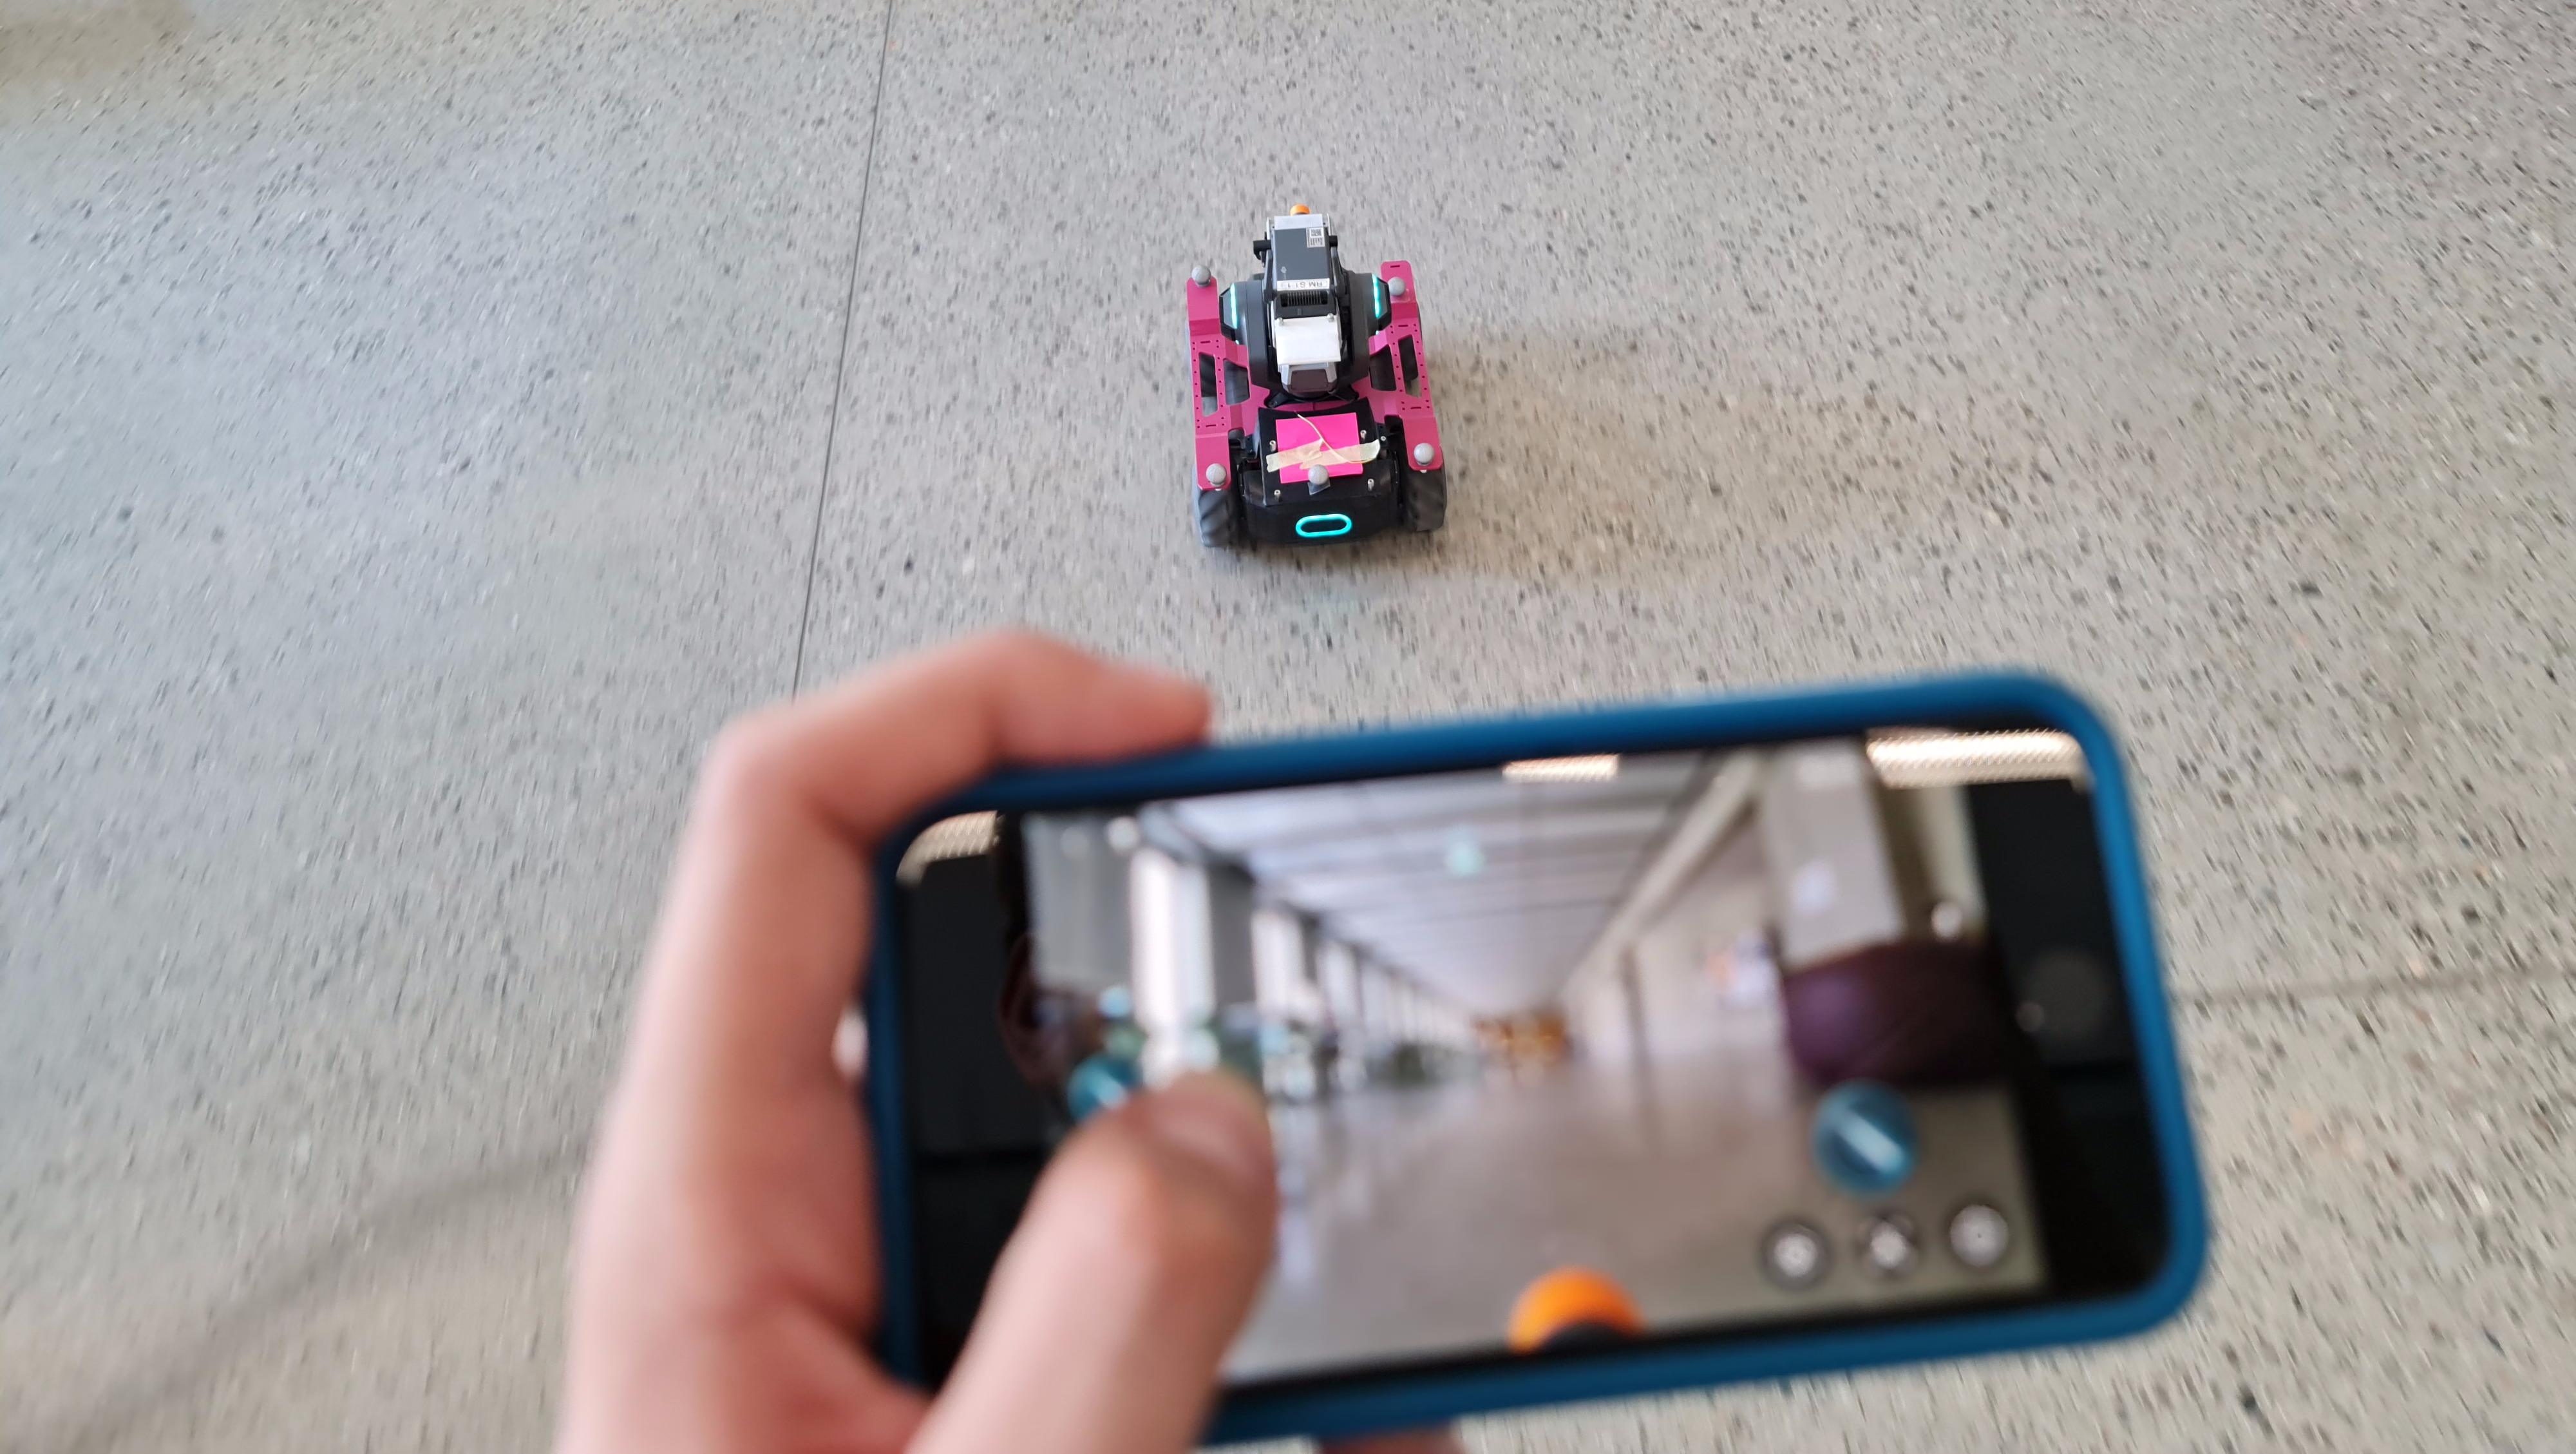
\includegraphics[width=0.97\textwidth]{img/data_coll.png}}
        \caption{Robomaster S1, picture shot during data collection.}
        \label{fig:data-coll}
    \end{figure}
    
    \section{Labeling}
        The videos are split into two groups: \emph{long} and \emph{short}, based on the video length.
        
        % \begin{figure}[htpb]
        %         \centering
        %         \centerline{\includegraphics[width=\textwidth]{img/labels/anomalies.png}}
        %         \caption{Robomaster S1, exploded-view from user manual with part names.}
        %         \label{fig:env-ex}
        % \end{figure}
        
        \subsection{Long videos}
        The long videos contain 5 classes. The labels are the following:

        % \begin{itemize}
        %     \item Human
        %     \item Lens dirty
        %     \item Object on Robot
        %     \item Object on Robot 2
        %     \item Normal
        % \end{itemize}

        % \begin{figure}[H]
        %     \centering
        %     \subfloat[]{
        %         \includegraphics[width=0.3\columnwidth]{img/labels/normal.png}
        %         \label{fig:label-normal}
        %         }
        %     \subfloat[]{
        %         \includegraphics[width=0.3\columnwidth]{img/labels/human.png}
        %         \label{fig:label-human}
        %         }
        %     \subfloat[]{
        %         \includegraphics[width=0.3\columnwidth]{img/labels/defects.png}
        %         \label{fig:label-defects}
        %         }
        %     \\
        %     \subfloat[]{
        %         \includegraphics[width=0.3\columnwidth]{img/labels/obj. on robot.png}
        %         \label{fig:label-obj-on-robot}
        %         }
        %     \subfloat[]{
        %         \includegraphics[width=0.3\columnwidth]{img/labels/obj. on robot2.png}
        %         \label{fig:label-obj-on-robot2}
        %         }
        %     \caption{Images for each corresponding label of the long section of the dataset}
        %     \label{fig:labels-long}
        % \end{figure}

        \subsubsection*{Normal}
            The normal class (\autoref{fig:label-normal}) contains frames where the camera is not obstructed by any object. The camera is clean and the robot's path is not obstructed.
            \begin{figure}[H]
                \centering
                \centerline{\includegraphics[width=0.75\textwidth]{img/labels/normal.png}}
                \caption{Robots\&Hazards dataset Corridors scenario, label normal}
                \label{fig:label-normal}
            \end{figure}

        \subsubsection*{Human}
            The human class (Figure \autoref{fig:label-human}) contains frames where a person is obstructing the robot's path. The person is usually standing in front of the robot and moves in the same direction as the robot.
            \begin{figure}[H]
                \centering
                \centerline{\includegraphics[width=0.75\textwidth]{img/labels/human.png}}
                \caption{Robots\&Hazards dataset Corridors scenario, label human}
                \label{fig:label-human}
            \end{figure}

        \subsubsection*{Defects}
            The defects class (\autoref{fig:label-defects}) contains frames where the camera has some kind of defect. The defect can be a scratch, a stain, or a fingerprint on the lens. This anomaly is simulated by placing an antistatic bag on the camera.
            \begin{figure}[H]
                \centering
                \centerline{\includegraphics[width=0.75\textwidth]{img/labels/defects.png}}
                \caption{Robots\&Hazards dataset Corridors scenario, label defects}
                \label{fig:label-defects}
            \end{figure}

        \subsubsection*{Object on Robot}
            The object on robot class (\autoref{fig:label-obj-on-robot}) contains frames where the robot \acrshort{fov} is obstructed by some kind of object fallen and stuck over the camera. \autoref{fig:sampei} shows the robot with the anomaly mounted on it.
            
             \begin{figure}[H]
                \centering
                \centerline{\includegraphics[width=0.75\textwidth]{img/labels/obj. on robot.png}}
                \caption{Robots\&Hazards dataset Corridors scenario, label Object on Robot}
                \label{fig:label-obj-on-robot}
            \end{figure}
            
            \begin{figure}[H]
                \centering
                \centerline{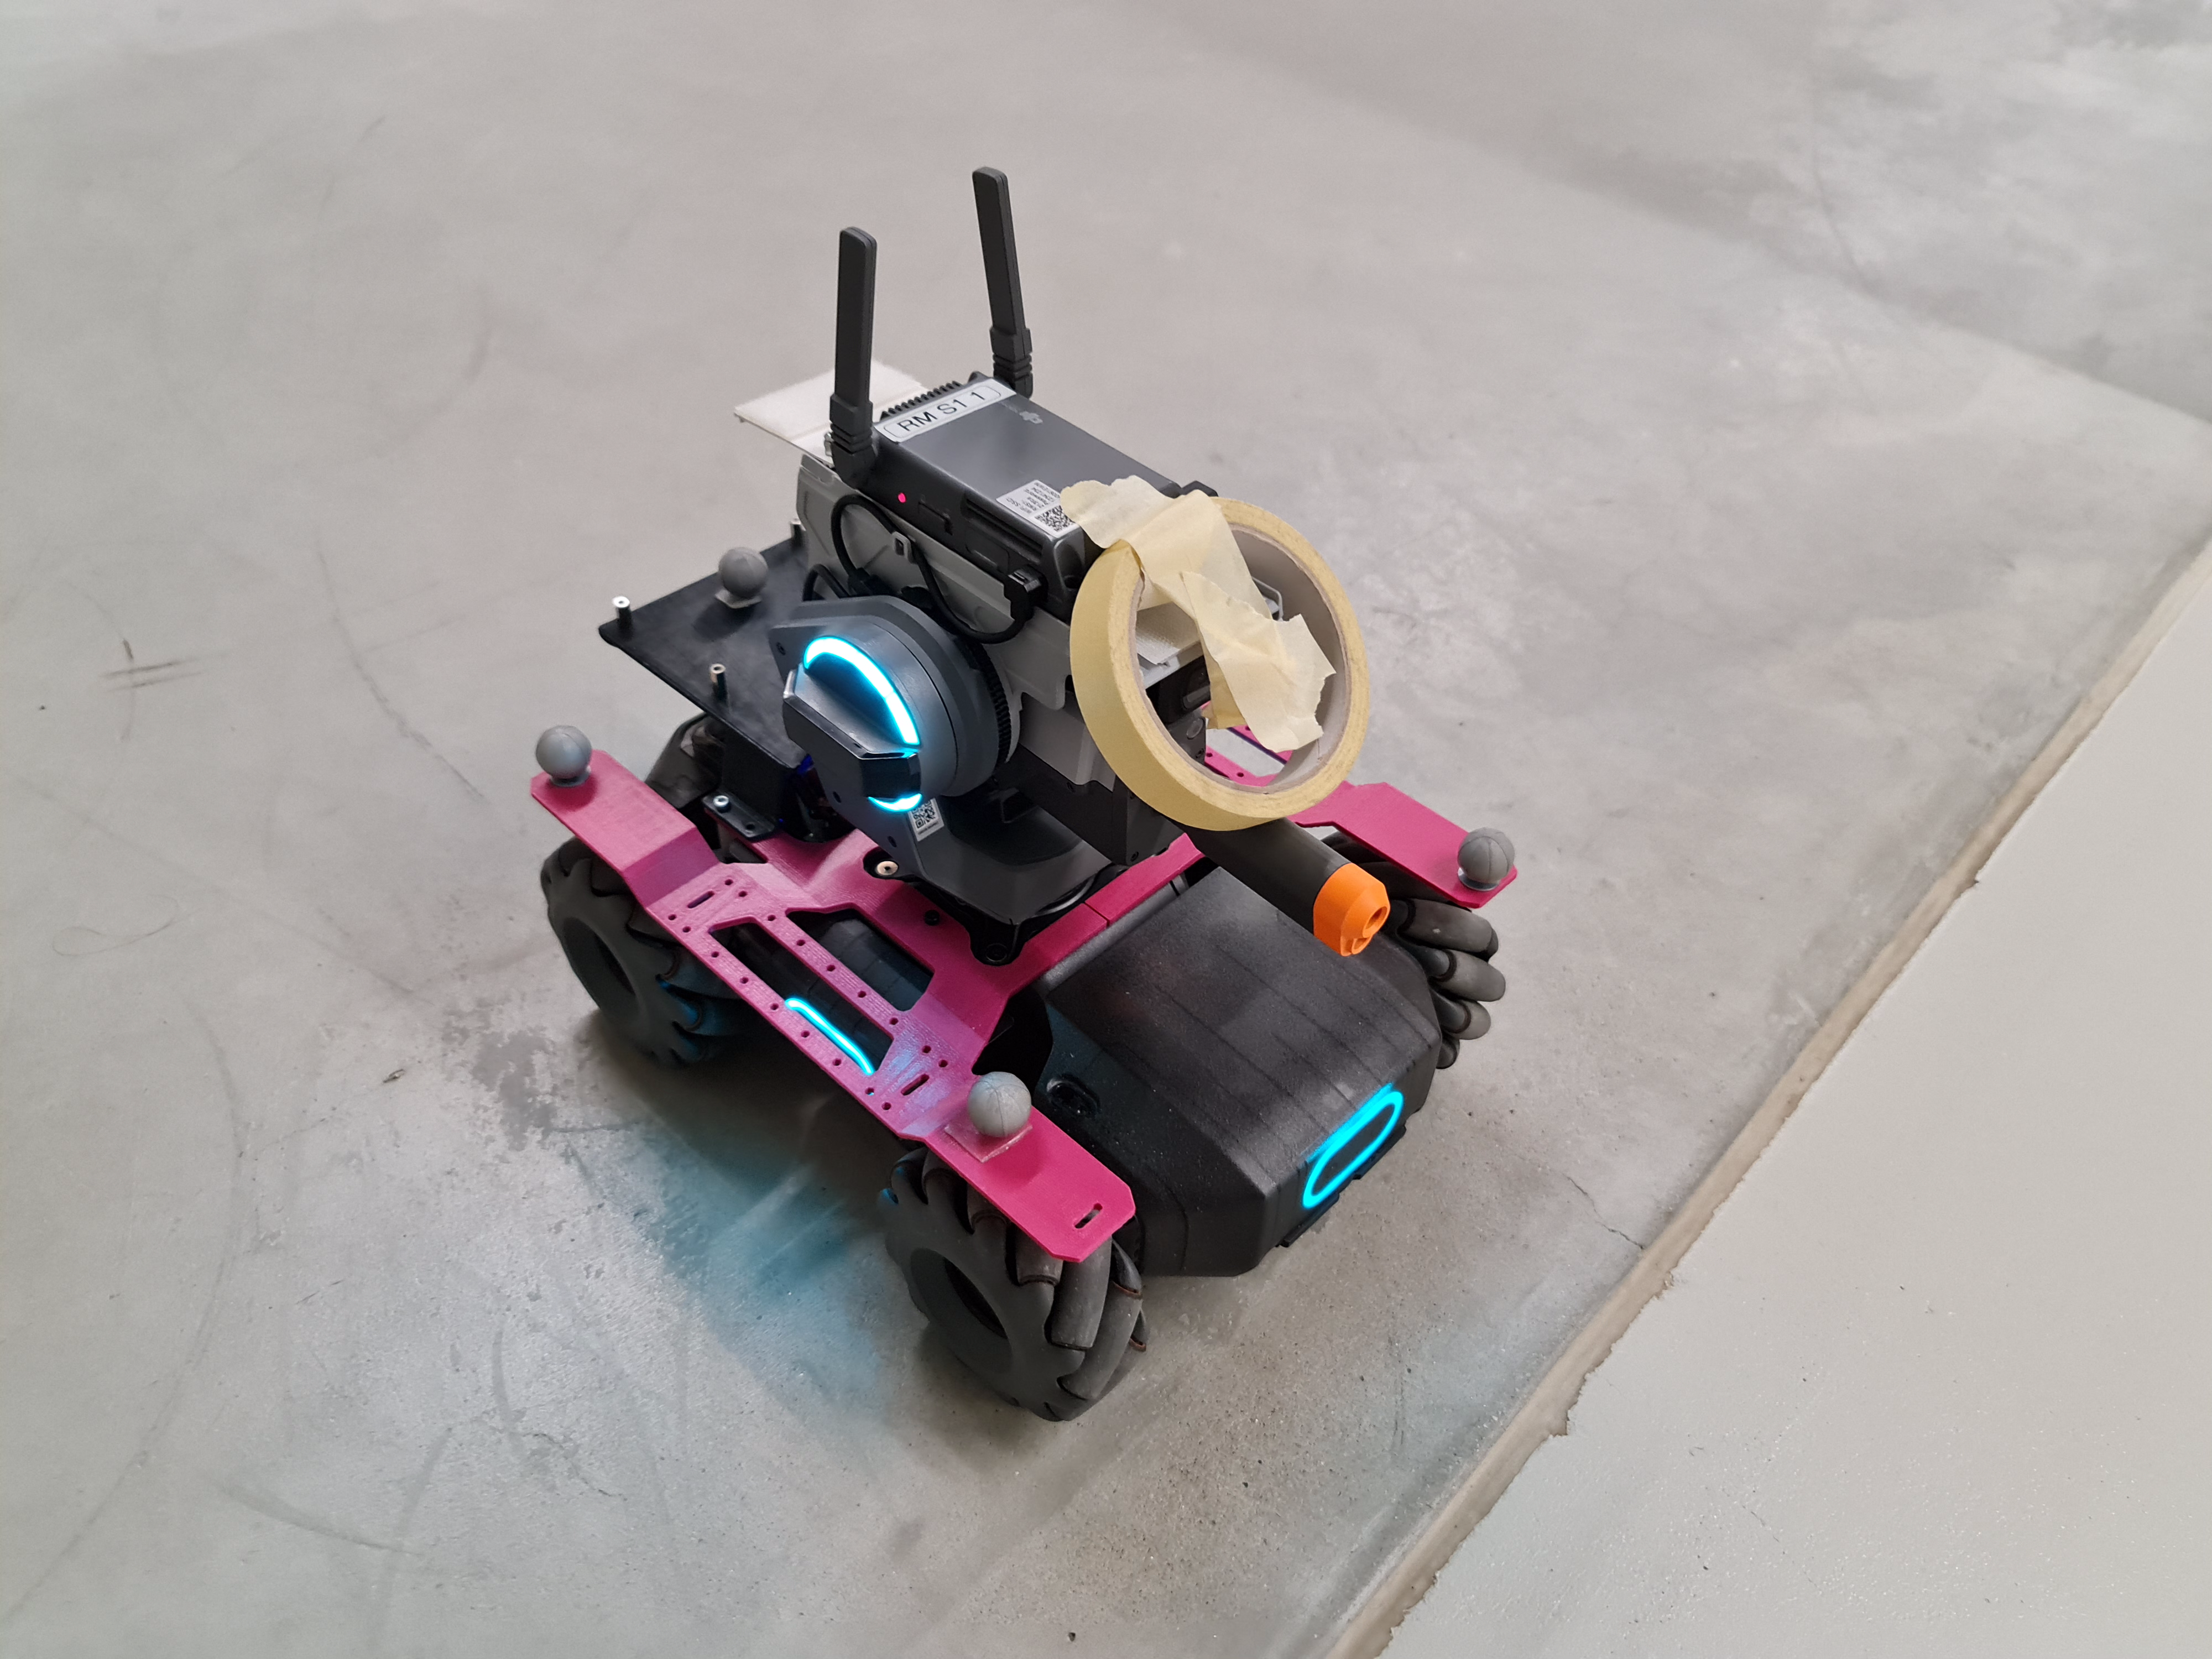
\includegraphics[width=\textwidth]{img/obj2_t.png}}
                \caption{Robomaster S1 mounted with the Object on robot anomaly}
                \label{fig:sampei}
            \end{figure}

        \subsubsection*{Object on Robot 2}
            This class is similar to the previous one, but the object is placed on the robot differently. The object is placed further in the camera in a way to only obstruct the central part of the robot's \acrshort{fov}. In \autoref{fig:sampei2} we can see the robot with the anomaly mounted on.
            \begin{figure}[H]
                \centering
                \centerline{\includegraphics[width=0.75\textwidth]{img/labels/obj. on robot2.png}}
                \caption{Robots\&Hazards dataset Corridors scenario, label Object on Robot 2}
                \label{fig:label-obj-on-robot2}
            \end{figure}
            
            \begin{figure}[H]
                \centering
                \centerline{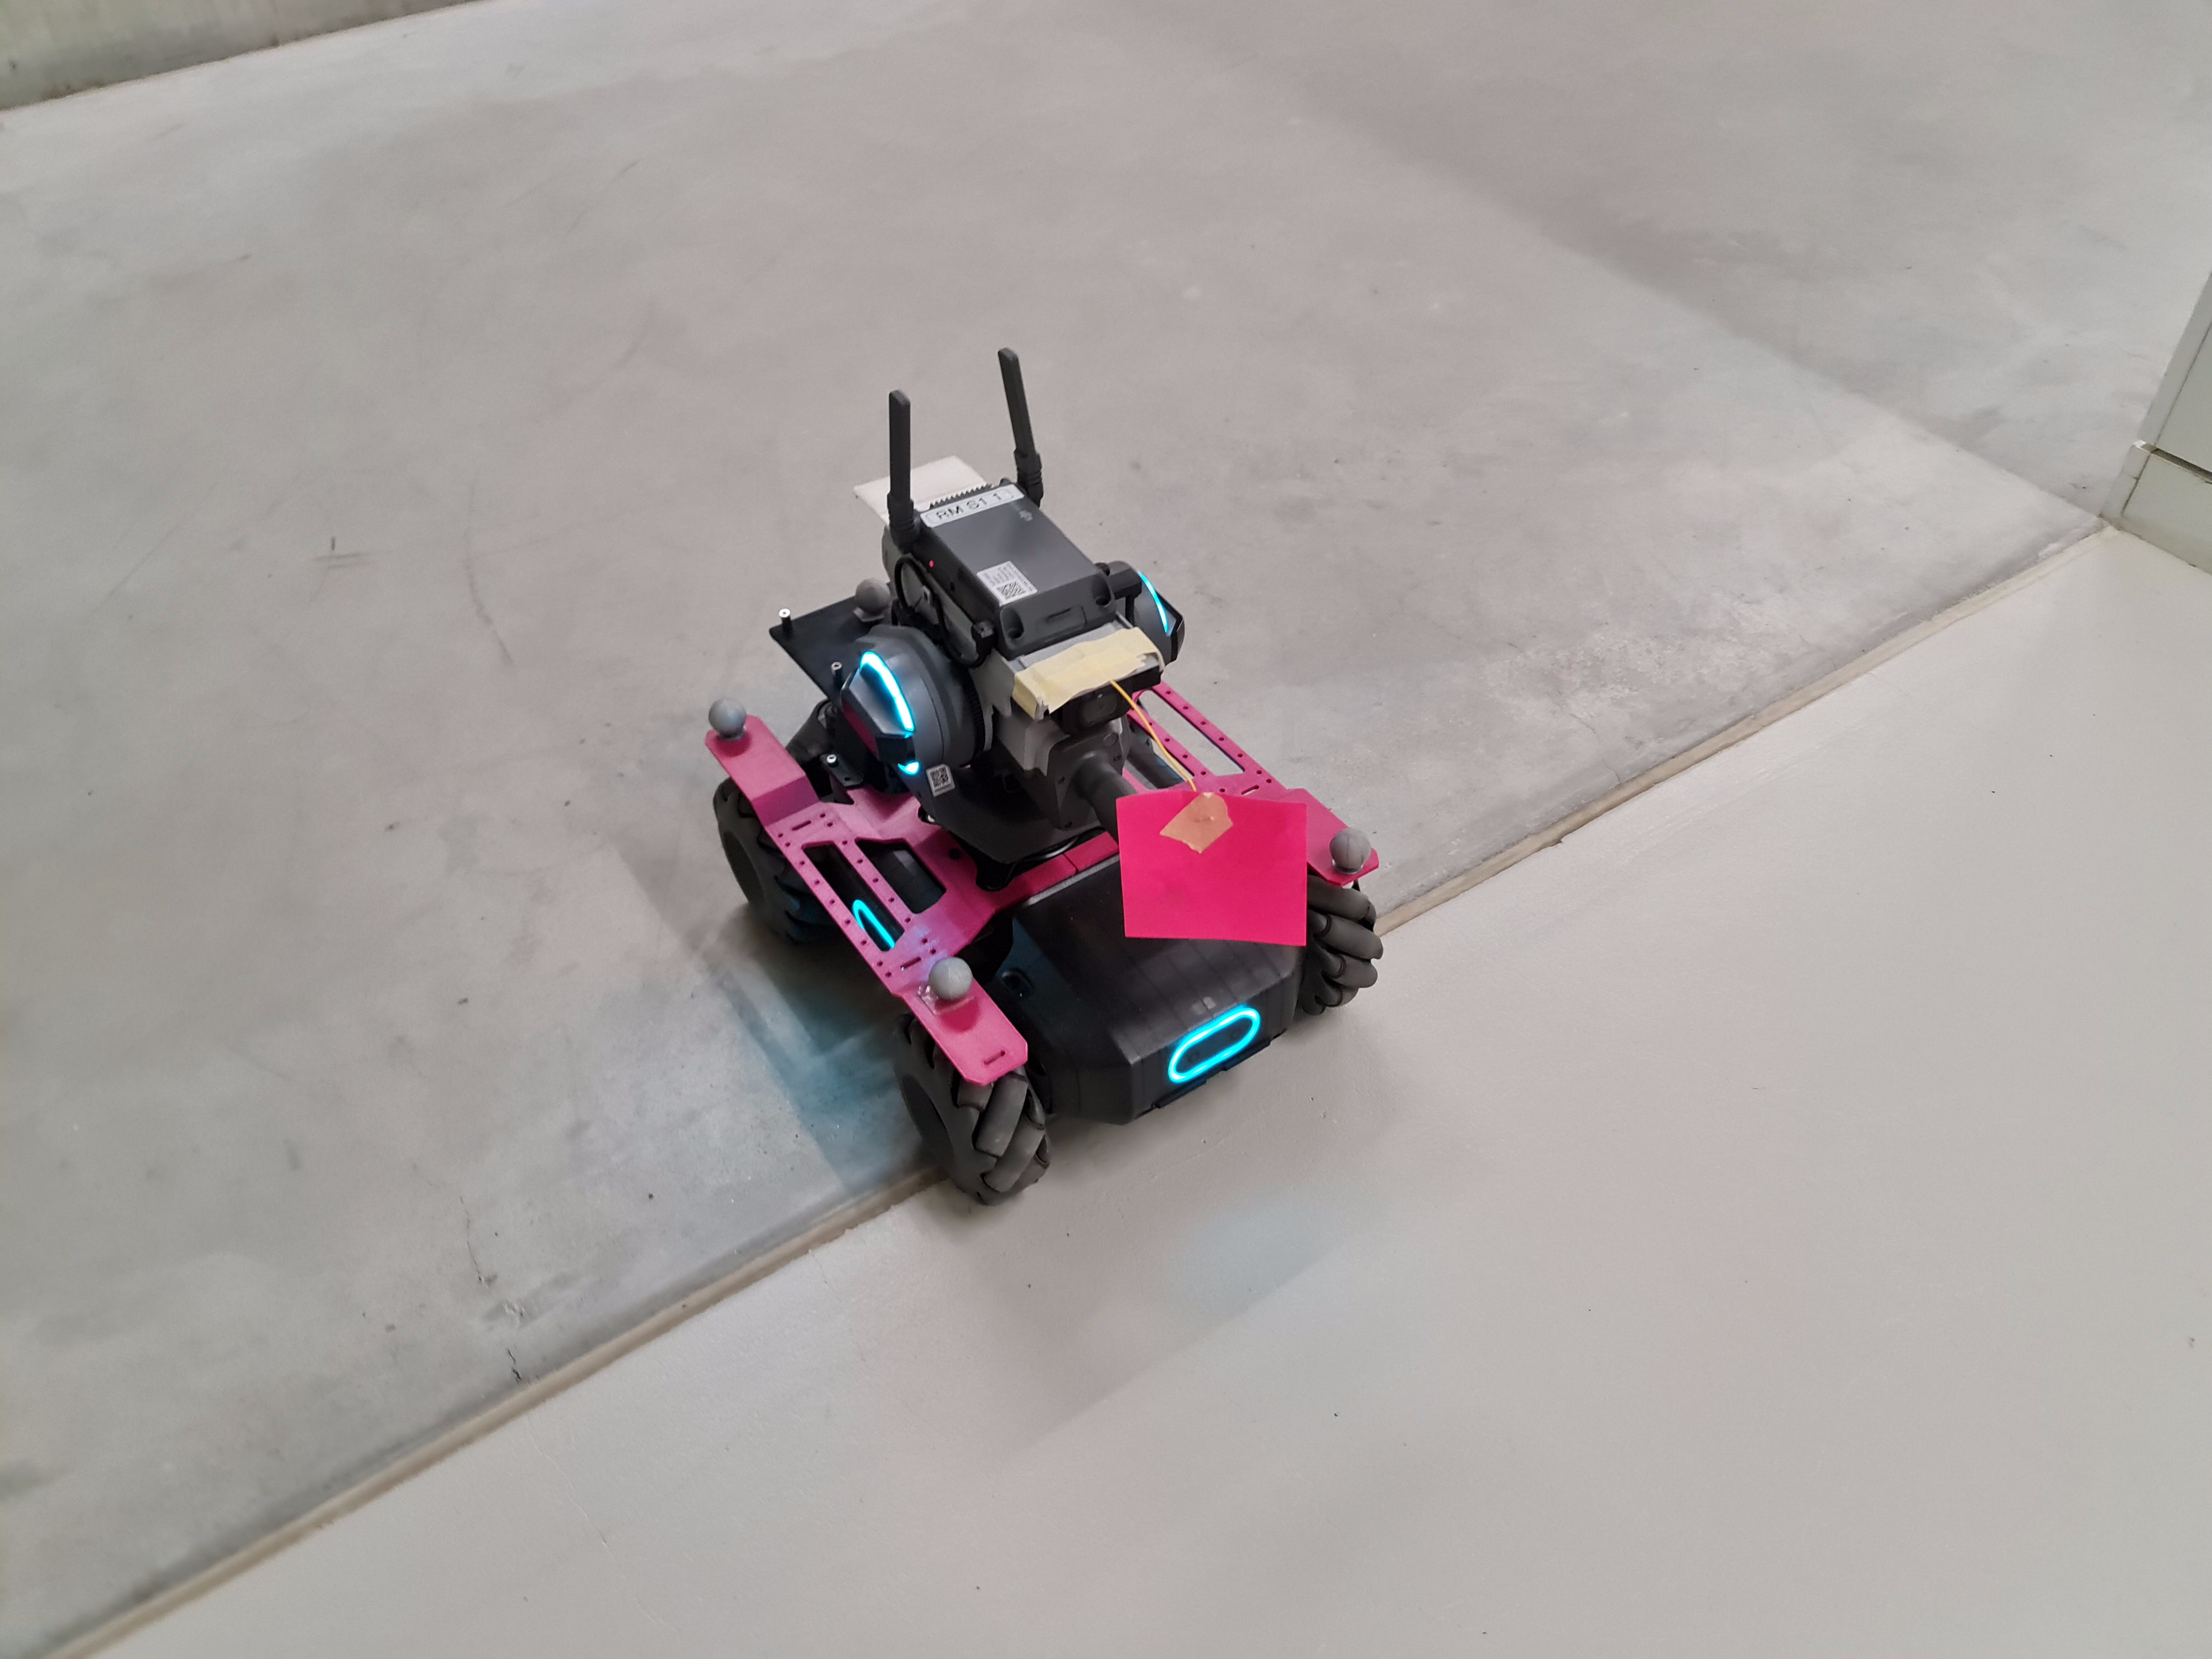
\includegraphics[width=\textwidth]{img/obj_th.png}}
                \caption{Robomaster S1 mounted with the Object on robot2 anomaly}
                \label{fig:sampei2}
            \end{figure}
        
        \subsection{Short videos}
        Short videos contain 7 classes. The labels are the following:
        % \begin{itemize}
        %     \item Cones
        %     \item Debris
        %     \item Floor
        %     \item Tape
        %     \item Trolley
        %     \item Cable
        %     \item Box
        % \end{itemize}
        % \begin{figure}[H]
        %     \centering
        %     \subfloat[]{
        %         \includegraphics[width=0.29\columnwidth]{img/labels/cones.png}
        %         \label{fig:label-cones}
        %         }
        %     \subfloat[]{
        %         \includegraphics[width=0.29\columnwidth]{img/labels/debris.png}
        %         \label{fig:label-debris}
        %         }
        %     \subfloat[]{
        %         \includegraphics[width=0.29\columnwidth]{img/labels/floor.png}
        %         \label{fig:label-floor}
        %         }
        %     \\
        %     \subfloat[]{
        %         \includegraphics[width=0.29\columnwidth]{img/labels/tape.png}
        %         \label{fig:label-tape}
        %         }
        %     \subfloat[]{
        %         \includegraphics[width=0.29\columnwidth]{img/labels/trolley.png}
        %         \label{fig:label-trolley}
        %         }
        %     \subfloat[]{
        %         \includegraphics[width=0.29\columnwidth]{img/labels/cable.png}
        %         \label{fig:label-cable}
        %         }
        %     \\
        %     \subfloat[]{
        %         \includegraphics[width=0.29\columnwidth]{img/labels/box.png}
        %         \label{fig:label-box}
        %         }
        %     \caption{Images for each corresponding label of the short section of the dataset}
        %     \label{fig:labels-short}
        % \end{figure}

        \subsubsection*{Cones}
            The cones class (\autoref{fig:label-cones}) contains frames where the path is obstructed by cones. The cones are usually placed in front of the camera, but they can also be placed on the sides.
            \begin{figure}[H]
                \centering
                \centerline{\includegraphics[width=0.75\textwidth]{img/labels/cones.png}}
                \caption{Robots\&Hazards dataset Corridors scenario, label cones}
                \label{fig:label-cones}
            \end{figure}

        \subsubsection*{Debris}
            The debris class (\autoref{fig:label-debris}) contains frames where the camera is obstructed by some kind of debris. The debris can be a piece of concrete, a piece of wood, or a piece of plastic. This anomaly is simulated by placing in front of the robot a broken concrete slab. 
            \begin{figure}[H]
                \centering
                \centerline{\includegraphics[width=0.75\textwidth]{img/labels/debris.png}}
                \caption{Robots\&Hazards dataset Corridors scenario, label debris}
                \label{fig:label-debris}
            \end{figure}

        \subsubsection*{Floor}
            The floor class (\autoref{fig:label-floor}) contains frames where the path is obstructed by some floor anomaly. The anomaly is simulated by placing a carpet on the floor.
            \begin{figure}[H]
                \centering
                \centerline{\includegraphics[width=0.75\textwidth]{img/labels/floor.png}}
                \caption{Robots\&Hazards dataset Corridors scenario, label floor}
                \label{fig:label-floor}
            \end{figure}
        
        \subsubsection*{Tape}
            The tape class (\autoref{fig:label-tape}) contains frames where the path is obstructed by some tape placed at random heights, even higher than the robot's height.
            \begin{figure}[H]
                \centering
                \centerline{\includegraphics[width=0.75\textwidth]{img/labels/tape.png}}
                \caption{Robots\&Hazards dataset Corridors scenario, label tape}
                \label{fig:label-tape}
            \end{figure} 

        \subsubsection*{Trolley}
            The trolley class (\autoref{fig:label-trolley}) contains frames where the path is obstructed by a trolley. The trolley can be a small or large.
            \begin{figure}[H]
                \centering
                \centerline{\includegraphics[width=0.75\textwidth]{img/labels/trolley.png}}
                \caption{Robots\&Hazards dataset Corridors scenario, label trolley}
                \label{fig:an-trolley}
            \end{figure}

        \subsubsection*{Cable}
            The cable class (\autoref{fig:label-cable}) contains frames where the path is obstructed by a cable. The cable can be a power cable, a network cable, or a USB cable.
            \begin{figure}[H]
                \centering
                \centerline{\includegraphics[width=0.75\textwidth]{img/labels/cable.png}}
                \caption{Robots\&Hazards dataset Corridors scenario, label cable}
                \label{fig:an-cable}
            \end{figure}

        \subsubsection*{Box}
            The box class (\autoref{fig:label-box}) contains frames where the camera is obstructed by a box. The box can be of any size.
            \begin{figure}[H]
                \centering
                \centerline{\includegraphics[width=0.75\textwidth]{img/labels/box.png}}
                \caption{Robots\&Hazards dataset Corridors scenario, label box}
                \label{fig:an-box}
            \end{figure}
    
\chapter{Experiments and Results}
    \label{chap:experiments}
    
    In this chapter, we introduce the experimental setup and explain the conducted experiments and the obtained results.
    
    \section{Experimental setup}
        For each experiment, the training set is divided into three partitions: $A$, $B$, and $C$, each one with a predetermined size. $A$ and $B$ partitions will be used as the initial labeled training set, while $C$ will be used as the large \emph{unlabeled} pool.
        
        
        In case the number of samples in the obtained training set is less than the size of the entire training set (i.e., $|A| + |B| + |C|$), \emph{resampling} is performed. This makes for a fair comparison between the different \acrshort{al} approaches.
        
        
        More in detail, experiments are conducted by training and testing 10 runs off an autoencoder the \acrshort{al} techniques explained in \autoref{sub:al}.
        %  \begin{itemize}
             \subsection*{AL1}
             This baseline model does not use any \acrshort{al} method. The model is trained only on the $A$ and $B$ partitions of the training set.
             
             \subsection*{AL2}
             This is our second baseline model, it randomly queries $n$ samples from partition $C$. The final model is trained on partitions $A$, $B$, and the newly sampled data.
             
             \subsection*{AL3.1}
             This approach trains an intermediate model ($AL1$) using only the $A$ and $B$ partitions. It then uses this model to query the most anomalous $n$ samples from $C$ to be included in the new training set for the model. The final model is trained on the new extended set.
             
             \subsection*{AL3.2}
             This approach works similarly to $AL3.1$, although it uses another intermediate model:
                \begin{enumerate}
                    \item the most anomalous $n/2$ samples (wrt AL1) from partition $C$ are queried;
                    \item an intermediate (AL-tmp) model is trained on this new expanded dataset;
                    \item the final dataset is obtained by the AL-tmp training set plus the $n/2$ most anomalous samples (wrt AL-tmp).
                \end{enumerate}
                
             \subsection*{AL4 to AL8}
             All these approaches use $AL1$ as intermediate model to query the $n$ most \emph{informative} samples from partition $C$ following the criteria shown in \autoref{sub:al}.
        %  \end{itemize}

    \section{Model exploration}

        Preliminary tests are conducted to check whether the models were learning correctly.
        
        
        These tests are conducted by both checking the AUC of the models in the test set and by visualizing the reconstructed images. Figures \ref{fig:pred-mnist}, \ref{fig:pred-rm} show model predictions for a \emph{normal} and an \emph{anomalous} sample. The model can reproduce any normal sample with little to no error. However, if the model receives an anomalous sample, it will not be capable of reconstructing it correctly. This results in the "brighter" anomaly map in both Figures.
        
        \begin{figure}[H]
                \centering
                \centerline{\includegraphics[width=\textwidth]{img/prediction_MNIST.png}}
                \caption{Example of predictions from a model trained on MNIST. The input image on the left is from the normal class, while the other on the right is anomalous}
                \label{fig:pred-mnist}
        \end{figure}
        
    % \subsection{Tests for models learning average}
    
        \subsection{Early phase}
        
            In an early phase, we studied models with extreme architectural characteristics such as an autoencoder with no bottleneck. This was done to study the bottleneck size hyperparameter for the MNIST dataset shown in \autoref{sub:bn}.
        
            % Models with a bottleneck size of 0 are used on MNIST to find out which bottleneck size is the best for the task. Models with a bottleneck size of 0 should learn an average representation of the training data. This is because the bottleneck layer is removed and the model is forced to learn the average representation of the training data.
    
            % Debug runs are necessary for these models because, for the first runs, they were not learning as expected. This is because in the first versions of the autoencoder when a bottleneck size of $0$ is used, the decoder receives a tensor filled with $0$ values. These values would nullify the weights of the decoder and the model would not learn anything, the only parameter it could learn is the bias. This problem is solved by feeding the decoder a tensor filled with $1$ values. This way the decoder would correctly learn the average representation of the training data.
        
        \subsection{Dummy models}
        
            We test some dummy models to check whether our model evaluation pipeline is working correctly. To test it we developed and deployed three dummy models:
            \begin{itemize}
                \item DummyFalse
                \item DummyTrue
                \item DummyRandom
            \end{itemize}
            
            The first model predicts any sample as \emph{normal}, and the second predicts everything as \emph{anomalous}. The third model randomly chooses between the two classes for any given input.
            
            As expected the AUC of DummyFalse and DummyTrue is 0.5. For DummyRandom the boxplot in \autoref{fig:pred-dummy} shows this model has an AUC score close to 0.5.
            
            \begin{figure}[H]
                \centering
                \centerline{\includegraphics[width=0.5\textwidth]{img/results/dummy.png}}
                \caption{Test AUC for DummyRandom model, boxplot of 18 runs.}
                \label{fig:pred-dummy}
            \end{figure}
            
            % \subsubsection{Early phase}
        
            % In an early phase we studied models with extreme architectural characteristics like an autoencoder with no bottleneck. This was done to study the hyperparameter for the MNIST dataset.
            % TODO: Descrivere e spiegare gli esperimenti baseline.
            % TODO: Insert average 3 prediction
        
    % \subsection{Baselines}
    %     TODO: Descrivere e spiegare gli esperimenti baseline.
    
    \section{Proxy task}
        %spiega che la proxy task é riprodurre al meglio l'input e che con questo task proxy l'autoencoder impara a estrarre le features e riprodurre l'input. noi poi sfruttiamo l'errore per risolvere la nostra vera task ovvero l'anomaly detection.
        We use the MNIST dataset for a \emph{proxy} task to perform \acrshort{ad}. We achieve this by using one class (3 in our case) of the dataset as normal. All the other classes are considered \emph{anomalous}.
        
        With this proxy task, the autoencoder learns how to extract the most useful features and reproduce the normal input as best as possible. We then exploit the computed error map to solve our real task which is \acrshort{ad}.

    \section{Experiments on MNIST}
        Most of the experiments are conducted on the \emph{proxy task} defined on the MNIST dataset. In this section we show the experiments and results obtained.
        \subsection{Bottleneck size}
        \label{sub:bn}
            One of the first experiments on MNIST is conducted to find the best bottleneck size for the task. 
            
            For simplicity and time constraints, this experiment is limited only to the approaches $AL1$, $AL2$, and $AL3.1$.
            It consists of training and testing 13 runs of models with different bottleneck sizes. The goal is finding the smallest bottleneck size which leads to the best results.
            
            For these experiments we test the following bottleneck sizes:
            \begin{itemize}
                \item 0, 1, 2, 4, 6, 8, 16, 32, 64, 128, 256, 512
            \end{itemize}
            The results are shown in \autoref{tab:bottleneck}.
            
            Based on the obtained results, we choose to use a bottleneck size of 64 for the next experiments with the MNIST dataset.
        
        % Please add the following required packages to your document preamble:
        % \usepackage{graphicx}
        \begin{table}[H]
        \centering
        \resizebox{\textwidth}{!}{%
        \begin{tabular}{l|l|lll|l|lll|l|l}
        \textbf{Model}   & \textbf{Mean} & \textbf{Stdev} &  & \textbf{Model}   & \textbf{Mean} & \textbf{Stdev} &  & \textbf{Model}     & \textbf{Mean} & \textbf{Stdev} \\ \cline{1-3} \cline{5-7} \cline{9-11} 
        \textbf{AL1-0}   & 0.813         & 0.186          &  & \textbf{AL2-0}   & 0.863         & 0.000          &  & \textbf{AL3.1-0}   & 0.866         & 0.001          \\
        \textbf{AL1-1}   & 0.880         & 0.004          &  & \textbf{AL2-1}   & 0.882         & 0.004          &  & \textbf{AL3.1-1}   & 0.887         & 0.004          \\
        \textbf{AL1-2}   & 0.882         & 0.004          &  & \textbf{AL2-2}   & 0.900         & 0.003          &  & \textbf{AL3.1-2}   & 0.901         & 0.004          \\
        \textbf{AL1-4}   & 0.900         & 0.003          &  & \textbf{AL2-4}   & 0.918         & 0.004          &  & \textbf{AL3.1-4}   & 0.921         & 0.004          \\
        \textbf{AL1-8}   & 0.918         & 0.004          &  & \textbf{AL2-8}   & 0.937         & 0.005          &  & \textbf{AL3.1-8}   & 0.942         & 0.002          \\
        \textbf{AL1-16}  & 0.953         & 0.006          &  & \textbf{AL2-16}  & 0.958         & 0.005          &  & \textbf{AL3.1-16}  & 0.966         & 0.003          \\
        \textbf{AL1-32}  & 0.964         & 0.005          &  & \textbf{AL2-32}  & 0.970         & 0.005          &  & \textbf{AL3.1-32}  & 0.976         & 0.003          \\
        \textbf{AL1-64}  & 0.966         & 0.005          &  & \textbf{AL2-64}  & 0.973         & 0.004          &  & \textbf{AL3.1-64}  & 0.979         & 0.003          \\
        \textbf{AL1-128} & 0.967         & 0.005          &  & \textbf{AL2-128} & 0.975         & 0.004          &  & \textbf{AL3.1-128} & 0.979         & 0.003          \\
        \textbf{AL1-256} & 0.968         & 0.006          &  & \textbf{AL2-256} & 0.974         & 0.006          &  & \textbf{AL3.1-256} & 0.979         & 0.003          \\
        \textbf{AL1-512} & 0.966         & 0.006          &  & \textbf{AL2-512} & 0.975         & 0.004          &  & \textbf{AL3.1-512} & 0.979         & 0.004         
        \end{tabular}%
        }
        \caption{Bottleneck research results. From left to right: Results for AL1 models, results for AL2 models, and results for AL3 models. The average and standard deviation are computed over 13 runs.}
        \label{tab:bottleneck}
        \end{table}

        \subsection{Bottleneck activation function}
            The second set of experiments is conducted to find the best activation function for the bottleneck layer.
            
            The experiment is conducted by performing 10 runs of models with different bottleneck size activations. For simplicity, we limited the experiment only to the approaches $AL1$, $AL2$, and $AL3$.
            
            
            We tested some of the most used activation functions:
            \begin{itemize}
                \item Sigmoid
                \item ReLu
                \item tanh
                \item no activation (linear)
            \end{itemize}
            
            
            \noindent The results of this experiment are shown in \autoref{fig:activation_test}.
            \\
            \\
            The models with a linear bottleneck performed better than the others, with lower variance and a higher average \acrshort{auc}.
            
            From now on we will only use models with a linear bottleneck layer.
            
             \begin{figure}[H]
                \centering
                \centerline{\includegraphics[width=\textwidth]{img/results/test_act.png}}
                \caption{Test AUC for the bottleneck activation function experiment on the MNIST dataset.}
                \label{fig:activation_test}
            \end{figure}
            
        \subsection{Data split}
            Once the bottleneck size and the bottleneck activation are found, the next step is finding the best partition sizes for the task.
            
            The experiment is conducted by performing 10 runs of models with different bottleneck data splits. For simplicity, we limited the experiment only to the approaches $AL1$, $AL2$, and $AL3$.
            
            We try the following splits:
            \begin{enumerate}
                \item 100 ($|A| = 50$, $ |B| = 50$, $|C| = 100$)
                \item 200 ($|A| = 100$, $ |B| = 100$, $|C| = 200$)
                \item 400 ($|A| = 200$, $ |B| = 200$, $|C| = 400$)
                \item 1000 ($|A| = 1000$, $ |B| = 1000$, $|C| = 2000$)
                \item 2000 ($|A| = 2000$, $ |B| = 2000$, $|C| = 4000$)
            \end{enumerate}
            
            The results of this experiment are shown in \autoref{fig:split_minst}. Based on the obtained results, we choose to use a data splitting of $1000$ images for the partitions $A$ and $B$ and $2000$ images for $C$.
            \begin{figure}[H]
                \centering
                \centerline{\includegraphics[width=\textwidth]{img/results/split_MN.png}}
                \caption{Test AUC for the partition size experiment on the MNIST dataset.}
                \label{fig:split_minst}
            \end{figure}

    \section{Experiments on the Hazards\&Robots dataset, Corridors scenario}
        Similar experiments are conducted on the real-life Hazards\&Robots dataset, Corridors scenario. This dataset is larger than MNIST, thus experiments require more time. Because of this, experiments in this section are not as broad as on the \emph{proxy} task.
        
        
        For the following experiments we perform \emph{data augmentation} along with resampling.
        
        We perform the following augmentation operations:
        \begin{itemize}
            \item Horizontal flip with a probability of 0.5;
            \item Random brightness contrast with a probability of 0.5, brightness and contrast limits of 0.1;
            \item Random crop with a probability of 0.5;
            \item Random rotation of maximum 10° with 0.5 probability.
        \end{itemize}
        \subsection{Early phase}
            In an early phase, we adapted the autoencoder to work with the images from the Hazards\&Robots, we then run some preliminary tests to check the correct function of the model (\autoref{fig:pred-rm}).
            
            \begin{figure}[H]
                \centering
                \centerline{\includegraphics[width=\textwidth]{img/prediction_RM.png}}
                \caption{Example of predictions from a model trained on the Hazards\&Robots dataset. The input image on the left is from the normal class, while the other on the right is anomalous}
                \label{fig:pred-rm}
            \end{figure}
            
        \subsection{Bottleneck size}
            We choose to use a bottleneck size of 16 because Mantegazza et al~\cite{mantegazza2022sensing} in their experiments on this dataset show it performs better.
            
        \subsection{Data split}
            The next step is finding the best partition size for this task.
            
            Because of time constraints, since experiments on this dataset require more time than MNIST, we only try the following splits to $AL1$ only:
            
            \begin{itemize}
                \item 2 ($|A| = 1$, $ |B| = 1$, $|C| = 2$)
                \item 20 ($|A| = 10$, $ |B| = 10$, $|C| = 20$)
                \item 200 ($|A| = 100$, $ |B| = 100$, $|C| = 200$)
                \item 2000 ($|A| = 1000$, $ |B| = 1000$, $|C| = 2000$)
            \end{itemize}
            
            \noindent We choose to add to the comparison two more experiments: $AL1-2$, and $AL1-2000$ with no image augmentation.
            
            
            The results in \autoref{fig:split_rm} show how effective the data augmentation is when the training set is small, with $AL1-2$ outperforming its version with no augmentation. On the other hand, for the models with an initial training set of 2000 images, the augmentation led to a very small decrease in the model performance. We suppose this small decrease is due to noise introduced by the process of augmentation.
            
            
            We choose to use a data splitting of $1000$ images for the splits $A$ and $B$ partitions and $2000$ images for partition $C$.
            
            \begin{figure}[H]
                \centering
                \centerline{\includegraphics[width=\textwidth]{img/results/split_RM.png}}
                \caption{Test AUC on the Hazards\&Robots dataset for different data split.}
                \label{fig:split_rm}
            \end{figure}
        
    \section{AL metrics comparison}
        Now we have the best bottleneck and data partition hyperparameters for both our tasks.
        The final experiments are conducted to test and compare the different \acrshort{al} approaches proposed in \autoref{sub:al}.
    
        \subsection{MNIST}
            The results of the final experiments on the proxy task are shown in \autoref{fig:comparison-MN}.
            From the chart, we notice that no $AL$ approach has outperformed the others in a significant way. We notice that even with the random approach there is a significant improvement over the baseline model ($AL1$). However, for this task, the \acrshort{al} approaches proposed do not provide any significant improvement over the random query method ($AL2$).
            
            We suppose this is because the MNIST dataset is too simple for this task, the model quickly learns which features to extract to correctly reconstruct the input. Thus finding clever solutions to query useful data for the model shows little to no improvements in this setup.
            
            \begin{figure}[H]
                \centering
                \centerline{\includegraphics[width=\textwidth]{img/results/final_MNIST.png}}
                \caption{Test AUC on final experiments on the MNIST dataset}
                \label{fig:comparison-MN}
            \end{figure}
        
        \subsection{Hazards\&Robots dataset, Corridors scenario}
            The results of the final experiments on the Hazards\&Robots dataset, Corridors scenario are shown in \autoref{fig:comparison-MN}.
            
            
            From this real-life dataset, the results show a different pattern. We still have significant improvements with any model compared to the baseline. However, in this case, we have some models outperforming the random. More in detail, the approach $AL8$ outperformed both the baselines ($AL1$, $AL2$), scoring an \acrshort{auc} close to the upper bound of the dataset while using a training set of only 4,000 images.
            
            Another trend we notice is that methods that work on the \acrshort{ae}'s latent space show better performance than the ones which work in the image space.
            
            \begin{figure}[H]
                \centering
                \centerline{\includegraphics[width=\textwidth]{img/results/final_Hazards&Robots.png}}
                \caption{Test AUC on final experiments on the Hazards\&Robots dataset, Corridors scenario.}
                \label{fig:comparison-RM}
            \end{figure}
            
        \subsection{Comparison}
            We now directly compare the final results for both tasks. \autoref{fig:comparison} shows an overview of the \acrshort{auc} for both the MNIST dataset and the Hazards\&Robots dataset, Corridors scenario.
            
            We immediately notice that the results for MNIST are more "compact" when compared to our real-life dataset. This encourages our hypothesis that the MNIST dataset is way too simple for the task, nullifying the effort of performing \acrshort{al}.
            
            On the other hand, the chart of results on the Hazards\&Robots dataset, Corridors scenario shows how \acrshort{al} can be effective when applied to more complex tasks, leading to an \acrshort{auc} close to the upper bound using only a small fraction of the training data.
            \begin{figure}[H]
                \centering
                \centerline{\includegraphics[width=\textwidth]{img/results/final_comparison.png}}
                \caption{Test AUC for final experiments. Comparison between MNIST and the Hazards\&Robots dataset, Corridors scenario}
                \label{fig:comparison}
            \end{figure}
            
        \subsection{Discussion}
        In this chapter we found the best bottleneck size, split size, and data split for both our tasks. We then tested the proposed \acrshort{al} approaches to both our datasets.
        
        
        \noindent We found out that for MNIST the best bottleneck size is 64, while 16 resulted the best for the Hazards\&Robots dataset.
        
        
        \noindent A linear bottleneck for the autoencoder leads to better performance then using an activation function.
        
        
        \noindent For both the datasets, the best split is 1000 images for partitions $A$ and $B$, 2000 for partition $C$.
        
        \noindent The approaches and the testing pipeline are validated using and testing some dummy models.
        
        \noindent As for the \acrshort{al} approaches, MNIST turned out to be way too simple for the task, with \acrshort{al} not providing any significant performance boost. On the other hand, on the Hazards\&Robots dataset the \acrshort{al} approaches which work in the latent space of the \acrshort{ae} outperformed the baselines and performed better than the \acrshort{al} methods which work in the image space.
        
        \noindent To summarize, \acrshort{al} applied the Hazards\&Robots dataset let us reach performance near to the upper bound by using only 4,000 samples.
        
        
% \include{chapters/6-Results}
\chapter{Conclusions}
\label{chap:conclusions}

% Punti chiave:
% Approcci AL si sono dimostrati funzionanti (battuto AL1) 
% AL6 e AL8 sono gli approcci con variabilità maggiore su MNIST 
% Al8 (Min-Max + anomaly score) è approccio più promettente per Campus, mentre per MNIST AL4 ha avuto I risultati migliori 
% MNIST si è dimostrato un dataset molto semplice, dove AL probabilmente non è necessario
% Miglioramenti su campus dataset più marcati rispetto a MNIST 
% Dati e approcci verificati anche con baseline dummy  
% Esplorata complessitá dataset RM considerando meno campioni 

 

 

% Ha senso usare AL? 
% MNIST lo conferma 
% Quale è l’approccio migliore? 
% MNIST non lo dice 
% Se MNIST non lo fornisce ha senso cercare su un dataset più complesso? 
% Sì 
% Si nota qualche trend sul dataset Campus? 
% Si nota che i modelli che fanno sampling sull’embedding performano meglio 
% Data augmentation influisce sui risultati? 
% Augmentation porta a performance + alte di base  

The objective of this work is to study \acrfull{al} techniques applied to \acrfull{ad} to reduce the training data while retaining similar performance on the test set.
\\

To achieve this we first build an \acrshort{ad} model inspired by the work done at \acrfull{idsia}. We then research the literature to find the metrics used for \acrshort{al} and explain them. After the literature research, we define our problem and design our solutions. We extend a real-life dataset for \acrshort{ad} with new samples collected using a ground robot with a front-facing camera. Then we perform our experiments on both a \emph{proxy} task defined on the MNIST dataset and the previously extended real-life dataset.
\\  
    
Our results show that on MNIST no \acrshort{al} approach has outperformed the others in a significant way. We assume this happened because MNIST is too simple for this task. On the other hand, for the dataset that we have collected, the most performing approach among all tested is the hybrid min-max with anomaly score. It reaches an \acrfull{auc} close to the upper bound model with only a small fraction of the training set. In the real-life dataset, we notice that the \acrshort{al} approaches that work on the latent space of the \acrfull{ae} outperform the approaches that work in the image space.

\section{Future Works}
The results of this work show that the proposed \acrshort{al} approach is viable for \acrshort{ad} applications in the context of mobile robots. To further improve the work we suggest the following:

\begin{itemize}
    \item \textbf{More Complex Models}:
    In this work, we have only used a simple \acrfull{ae}. It is possible to use more complex models such as \acrfull{vae} or Real-NVP based models to see if they can achieve better results.
    \item \textbf{More Challenging Dataset}:
    The Corridor scenario of the dataset we used turned out not to be very challenging. Testing the \acrshort{al} approaches in more challenging scenarios would be interesting to test the approaches on a more difficult real-life setting.
    \item \textbf{Transfer Learning techniques}:
    In this work, we have used the real-life dataset as a single Domain. However real-life scenarios are often diverse. It would be interesting to test our AL solution while keeping in consideration Domain Adaptation.
\end{itemize}

\appendix %optional, use only if you have an appendix

% \chapter{More figures and tables}
\fontsize{9}{9}\selectfont
\chapter{Code}
\label{chap:code}

\section{Autoencoder classes}
\subsection{Autoencoder}
\lstinputlisting[language=Python]{code/autoencoder.py}

\subsection{Convolutional encoder}
\lstinputlisting[language=Python]{code/convolutional_encoder.py}

\subsection{Bottleneck}
\lstinputlisting[language=Python]{code/bottleneck.py}

\section{Dataset classes}
\subsection{Dataset Handler}
\lstinputlisting[language=Python]{code/dataset_handler.py}
\subsection{Dataset}
\lstinputlisting[language=Python]{code/dataset.py}

\section{Utility Scripts}
\subsection{Function get_most_anomalous}
\lstset{language=python}
\begin{lstlisting}
def get_most_anomalous(model, data, n=100, criterion=None):
    device = torch.device("cuda:0" if torch.cuda.is_available() else "cpu")
    model.eval()
    loss_fn = torch.nn.L1Loss()
    losses = []
    dataloader = torch.utils.data.DataLoader(data, batch_size=1, shuffle=True,
                                             pin_memory=True, num_workers=4)
    with torch.no_grad():
        for frame, _ in tqdm(dataloader):
            frame = frame.to(device)
            enc, dec = model(frame)
            loss = loss_fn(frame, dec)
            losses.append(loss.item())

    idx = np.argsort(losses)[::-1][:n]
    return torch.utils.data.Subset(data, idx), idx
\end{lstlisting}

\subsection{Function get_most_informative}
\lstset{language=python}
\begin{lstlisting}
def get_most_informative(model, data, train_data, n=100, criterion="error_map"):
    '''
    Return the n most informative frames,
    informativeness score based on model uncertainty
    '''
    device = torch.device("cuda:0" if torch.cuda.is_available() else "cpu")
    dataloader = torch.utils.data.DataLoader(data, batch_size=64, shuffle=True,
                                             pin_memory=True, num_workers=4)
    train_loafer = torch.utils.data.DataLoader(train_data, batch_size=64,
                                               shuffle=True, pin_memory=True,
                                               num_workers=4)
    model.eval()

    latent_spaces = []
    train_latent_spaces = []

    with torch.no_grad():
        for frame, _ in tqdm(dataloader):
            frame = frame.to(device)
            enc, dec = model(frame)
            for l_space in enc:
                latent_spaces.append(l_space.detach().cpu().numpy())
        for frame, _ in tqdm(train_loafer):
            frame = frame.to(device)
            enc, dec = model(frame)
            for l_space in enc:
                train_latent_spaces.append(l_space.detach().cpu().numpy())

    latent_spaces = np.array(latent_spaces)
    train_latent_spaces = np.array(train_latent_spaces)

    latent_spaces = (latent_spaces - train_latent_spaces.mean(
        axis=0)) / train_latent_spaces.std(axis=0)
    train_latent_spaces = (train_latent_spaces - train_latent_spaces.mean(
        axis=0)) / train_latent_spaces.std(axis=0)

    if criterion.lower() == "error_map":
        informativeness = []
        with torch.no_grad():
            for frame, _ in tqdm(dataloader):
                frame = frame.to(device)
                enc, dec = model(frame)
                for in_frame, decoded in zip(frame, dec):
                    error_map = np.clip(
                        abs(decoded.cpu().detach().numpy() -
                            in_frame.cpu().detach().numpy()),
                        0, 1)
                    anomaly_map = error_map.reshape(-1)
                    informativeness.append(np.mean(anomaly_map))

        idx = np.argsort(informativeness)[::-1][:n]

    elif criterion.lower() == "latent_distance":

        l_mean = np.mean(train_latent_spaces, axis=0)

        informativeness = [np.mean(np.abs(l_space - l_mean)) for l_space in
                           tqdm(latent_spaces)]
        idx = np.argsort(informativeness)[::-1][:2 * n]
        informativeness = []
        for i in tqdm(idx):
            info_score = 0
            l_space = latent_spaces[i]
            for j in idx:
                l_space_j = latent_spaces[j]
                info_score += np.linalg.norm(l_space - l_space_j).item()
            informativeness.append(info_score / len(idx))

        new_idx = np.argsort(informativeness)[::-1][:n]
        idx = idx[new_idx]

    elif criterion == "minmax":

        distances = distance_matrix(train_latent_spaces, latent_spaces)

        # most_distant_per_train = np.argmax(distances, axis=1)
        most_close_per_unlabel = np.argmin(distances, axis=0)
        closeness_per_unlabel = [np.argsort(distances[:, i]) for i in
                                 range(len(distances[0]))]
        print(np.max(most_close_per_unlabel))
        lst = [[] for _ in range(np.max(most_close_per_unlabel) + 1)]
        idx = [[] for _ in range(np.max(most_close_per_unlabel) + 1)]
        for i, p in enumerate(most_close_per_unlabel):
            lst[p].append(distances[p, i])
            idx[p].append(i)
        ids = []
        for i in range(len(lst)):
            if lst[i]:
                ids.append(np.argmax(np.array(lst[i])))
            else:
                ids.append(0)
                idx[i].append(np.argmax(distances[i, :]))
        new_idx = [idx[i][num] for i, num in zip(range(len(ids)), ids) if
                   num is not None]
        idx = new_idx[:n]

        informativeness = []

        sorted_dist = []
        sorted_idx = []

    elif criterion == "minmax_iterative":
        # distances = distance_matrix(train_latent_spaces, latent_spaces)
        dtree = cKDTree(train_latent_spaces)
        closest_point = dtree.query(latent_spaces, k=1)[1]
        distances = [minkowski_distance(p, nn) for p, nn in
                     zip(latent_spaces, closest_point)]
        original_ids = [i for i in range(len(latent_spaces))]
        idx = []

        with tqdm(total=n) as pbar:
            while len(idx) < n:
                chosen = np.argmax(distances)
                true_chosen = original_ids[chosen]
                original_ids = original_ids
                idx.append(true_chosen)
                pbar.update(1)
                l_space = latent_spaces[true_chosen]
                # latent_spaces = np.delete(latent_spaces, chosen, axis=0)
                original_ids.remove(true_chosen)
                distances.remove(distances[chosen])
                new_dists = [minkowski_distance(l_space, other) for other in
                             latent_spaces]
                distances = [min(d1, d2) for d1, d2 in
                             zip(distances, new_dists)]

    elif criterion == "minmax_iterative2":
        ds = cdist(train_latent_spaces, latent_spaces)
        ds = np.min(ds, axis=0)
        rs = []

        for _ in trange(n):
            i = np.argmax(ds)
            rs.append(i)
            nds = cdist(latent_spaces, latent_spaces[i:i + 1])[:, 0]
            ds = np.minimum(ds, nds)
        idx = rs

    elif criterion == "minmax_anomaly":
        ds = cdist(train_latent_spaces, latent_spaces)
        ds = np.min(ds, axis=0)
        idx = []
        samples = None
        rs = []

        print("Selecting samples from clusters")
        for _ in trange(3 * n):
            i = np.argmax(ds)
            rs.append(i)
            nds = cdist(latent_spaces, latent_spaces[i:i + 1])[:, 0]
            ds = np.minimum(ds, nds)
        idx = rs

        print("Selecting most anomalous samples")
        dataset = torch.utils.data.Subset(data, idx)
        data, idx = get_most_anomalous(model, dataset, n)
        return data

    else:
        raise ValueError("Criterion not supported")
    return torch.utils.data.Subset(data, idx)
\end{lstlisting}
\fontsize{12}{12}\selectfont


\backmatter


% \chapter{Glossary} %optional
\printnoidxglossary[type=\acronymtype,title=Acronyms]
% \printnoidxglossaries[type=\acronymtype]

\clearpage

% \bibliographystyle{alpha}
% \bibliographystyle{dcu}
\bibliographystyle{plainnat}
\bibliography{biblio}

%\cleardoublepage
%\theindex %optional, use only if you have an index, must use
	  %\makeindex in the preamble

\end{document}
